% article_paper2.tex — Application companion to Paper 1 (HBMAE framework).
% Target: Journal of Nuclear Materials, regular article.
% Compile: tectonic article_paper2.tex (pdflatex broken in env).

\documentclass[11pt]{article}
\usepackage[margin=1in]{geometry}
\usepackage{amsmath,amssymb,amsthm}
\usepackage{mathtools}
\usepackage{graphicx}
\usepackage{hyperref}
\usepackage[round,authoryear]{natbib}
\usepackage{booktabs}
\usepackage{xspace}
\usepackage{siunitx}
\usepackage{caption}
\usepackage{longtable}
\usepackage{array}
\captionsetup{font=small,labelfont=bf}

% Minimal theorem environment (used sparingly here; main proofs live in Paper 1).
\theoremstyle{plain}
\newtheorem{theorem}{Theorem}
\newtheorem{proposition}[theorem]{Proposition}
\theoremstyle{definition}
\newtheorem{definition}{Definition}
\theoremstyle{remark}
\newtheorem{remark}{Remark}

% Notation shortcuts (kept consistent with Paper 1).
\newcommand{\eS}{\ensuremath{e_{\mathrm{s}}^{-}}\xspace}
\newcommand{\eAq}{\ensuremath{e_{\mathrm{aq}}^{-}}\xspace}
\newcommand{\Clt}{\ensuremath{\mathrm{Cl}_2^{\bullet-}}\xspace}
\newcommand{\Brt}{\ensuremath{\mathrm{Br}_2^{\bullet-}}\xspace}
\newcommand{\It}{\ensuremath{\mathrm{I}_2^{\bullet-}}\xspace}
\newcommand{\Xt}{\ensuremath{\mathrm{X}_2^{\bullet-}}\xspace}
\newcommand{\Cltdiss}{\ensuremath{\mathrm{Cl}_{2,\,\mathrm{diss}}}\xspace}
\newcommand{\HBMAE}{HBMAE\xspace}
\newcommand{\Ea}{E_a}
\renewcommand{\d}{\mathrm{d}}
\newcommand{\R}{\mathbb{R}}

\title{\bfseries A Calibrated Multi-Salt Radiolysis Model for Molten Chloride
       and Fluoride Reactor Fuels:\\
       Application of Hierarchical Bayesian Mechanism-Adequacy Estimation
       to Operational MSR Predictions}

\author{M.\ Tanore-Tamales \\
        \small Idaho National Laboratory, Idaho Falls, ID 83415, USA \\
        \small \texttt{mauricio.tanoretamales@inl.gov}}

\date{\today}

\begin{document}
\maketitle

\begin{abstract}
\noindent
The molten salt reactor (MSR) concept requires quantitative predictions of
how the salt's chemical inventory evolves under sustained radiation, on
timescales spanning nanoseconds through decades.  We construct a
calibrated multi-salt radiolysis model for chloride and fluoride MSR
fuels by combining a mechanistic reaction network with a digitized corpus
of pulse-radiolysis and chronic gamma-irradiation literature.  The
likelihood-bearing calibration corpus contains 73~observations drawn from
13~of the 14~digitized source papers in Table~\ref{tab:sources}.  The
model is calibrated through the Hierarchical Bayesian Mechanism-Adequacy
Estimation (\HBMAE) framework of our companion methodology
paper~\citep{Tanore2026PaperI}, summarized in
Section~\ref{sec:hbmae-brief}.  The integrated 24-parameter posterior
recovers the published Iwamatsu Arrhenius parameters for chromium and
zinc within $1\sigma$ and quantifies the Pikaev--Iwamatsu inter-facility
offset at $b^{(\mathrm{Pikaev})} = -3.35\,[-4.53,-2.44]$.  A
meta-hierarchical chemistry-feature regression on charge, ionic radius,
and electronegativity recovers in-corpus microsecond-Pikaev metals within
$\sim$1~log unit but under-predicts the LEAF-picosecond corpus by
2--4~log units; the regression is therefore descriptive rather than
predictive for fission-product elements whose operational chemistry is
not yet represented at any facility in the training set.
We deploy the calibrated model to two operational MSR design problems.
A 500~MW(th) NaCl-UCl\textsubscript{3} fast-spectrum reactor yields,
under the Phillips-bounded U(III)/U(IV) kernel, a posterior on cover-gas
$P_{\mathrm{Cl}_2}$ whose median lies far below a notional 100~Pa
screening threshold; this margin is dominated by the assumed U-redox
sink and would collapse if the U-buffer is incomplete
(\S\ref{sec:op:mcfr:ubuffer}).  A FLiBe-UF\textsubscript{4} salt loop
predicts a steady-state cover-gas $P_{\mathrm{F}_2}$ of 31~Pa (median;
90\,\% CI $[19,\,44]$~Pa), within a factor of three of the same screening
threshold and dominated by the Davis-2022 $G(\mathrm{F}_2)$ and the
Toth--Felker recombination $\Ea$ extrapolation from 423~K to 873~K.
Posterior variance attribution and three recommended experiments are
reported in Section~\ref{sec:operational}.
\end{abstract}

\noindent\textbf{Keywords:}
molten salt reactor;
radiolysis;
chloride salt;
fluoride salt;
NaCl--UCl\textsubscript{3};
FLiBe;
chemical kinetic network;
Bayesian calibration;
uncertainty quantification.

\bigskip

% =============================================================================
\section{Introduction}\label{sec:intro}
% =============================================================================

The molten salt reactor concept has re-emerged in the past decade as a leading
candidate for advanced fission heat generation, with active commercial
development of fast-spectrum chloride-fueled designs
\citep{Mausolf2024,TerraPower2021} and thermal-spectrum fluoride-cooled and
fluoride-fueled designs \citep{Forsberg2020,Andreades2014,Holcomb2012}.  Each
of these designs rests on a quantitative understanding of the chemical
evolution of the salt under sustained ionizing radiation.  At time scales
ranging from nanoseconds (solvated electrons and primary radical
recombination) through years (cumulative redox drift and accumulation of
gaseous radiolysis products in the cover-gas system), the salt chemistry
governs four engineering outcomes simultaneously:

\begin{enumerate}
\item the \emph{redox state} of the salt, which determines structural
      corrosion rates against Hastelloy, SS-316 and Mo--Re alloys
      \citep{Carotti2017,Olander2002};
\item the \emph{cover-gas inventory} of molecular Cl\textsubscript{2} in
      chloride systems or F\textsubscript{2} in fluoride systems, which
      governs off-gas system design and accident-source-term calculations
      \citep{Sohal2010,IAEA2013MSR};
\item the \emph{speciation of dissolved fission products}, in particular the
      partitioning of iodine, tellurium, and cesium between salt and cover
      gas, which determines containment release pathways
      \citep{Briggs1964,Williams2006};
\item the \emph{long-term thermophysical stability} of the salt itself,
      which determines fuel re-processing and salt cleanup requirements
      \citep{Romatoski2017,Yoshikawa2018}.
\end{enumerate}

The pulse-radiolysis literature that supplies the kinetic underpinnings of
this chemistry has grown substantially over the last five years.  The
Brookhaven LEAF program has produced quantitative kinetics for the solvated
electron \eS and the dichlorine radical anion \Clt in molten LiCl--KCl
eutectic at \SIrange{400}{600}{\celsius} \citep{Iwamatsu2022}, for
chromium-mediated electron transfer in the same melt
\citep{Iwamatsu2026}, for iodide perturbation of the chloride radical pool
\citep{Conrad2023}, for neodymium speciation as a representative lanthanide
\citep{CastroBaldivieso2026}, and for the first actinide rate constant in
chloride media (Cf\textsuperscript{3+} oxidation by \Clt and
SO\textsubscript{4}\textsuperscript{$\bullet-$}) \citep{Rotermund2024}.
Soviet-era pulse-radiolysis measurements
\citep{Pikaev1982,Makarov1982,Hagiwara1987} established the basic transient
inventory across the alkali-halide series at the order-of-magnitude level.
Ab~initio molecular dynamics
calculations~\citep{KristoffersenMetiu2018} provide
thermodynamic-feasibility anchors for the chloride redox sub-network.
Steady-state fluorine-gas yields from gamma-irradiated LiF, BeF\textsubscript{2},
UF\textsubscript{4}, ThF\textsubscript{4}, and FLiBe powders have been
recently quantified~\citep{Davis2022}, complementing the early Toth--Felker
recombination measurements~\citep{Toth1990}.  In the chloride-salt nuclear
fuel context, Phillips and coworkers~\citep{Phillips2022} reported the first
long-duration gamma-irradiation of NaCl-UCl\textsubscript{3} salt with no
detectable Cl\textsubscript{2} above approximately~\SI{1000}{ppm} after
\SI{31}{\mega\gray} of dose, providing a critical censored upper bound for
calibration.

Despite this experimental progress, no published compilation simultaneously
calibrates against the chloride and fluoride corpora in a single framework
within which an operational MSR designer can run an auditable,
uncertainty-quantified cover-gas Cl\textsubscript{2} or F\textsubscript{2}
prediction.  The available kinetic compilations are either single-paper
Arrhenius fits with no cross-host transferability, hand-tuned multi-paper
averages without formal calibration, or theoretical/AIMD computations that
have not been validated against an explicitly digitized multi-modality
corpus; Mausolf and coworkers~\citep{Mausolf2024} review the closest related
chloride compilation but do not perform a full multi-modality Bayesian
calibration.  This paper closes that gap.

The methodological backbone of the calibration is a hierarchical Bayesian
framework that jointly handles transient time-series, scalar rate constants,
derived Arrhenius pairs, one-sided censored detection limits, G-values, and
molar absorptivities, while resolving inter-facility systematic biases and
cross-host chemistry-feature transfer.  The full development is in our
companion methodology paper~\citep{Tanore2026PaperI}; we refer to that paper
for the formal theorems on identifiability and contraction and for the
synthetic-benchmark comparison against four state-of-the-art comparator
methods.  Section~\ref{sec:hbmae-brief} below summarizes the five-layer
construction sufficiently to read the present paper without consulting
Paper~I.  The present paper is the \emph{application} companion: we take
the calibrated 24-parameter \HBMAE\ posterior as given, extend it with a
chemistry-feature regression that supplies predictions for elements with
no pulse-radiolysis data, and deploy the resulting model to compute
screening-level operational predictions for both NaCl-UCl\textsubscript{3}
and FLiBe-UF\textsubscript{4} reactor concepts.

\subsection{HBMAE methodology in brief}\label{sec:hbmae-brief}

Hierarchical Bayesian Mechanism-Adequacy Estimation (\HBMAE) is a five-layer
Bayesian construction designed for kinetic networks calibrated against
heterogeneous, multi-facility, multi-host data.  We summarize the five
layers here so that the operational predictions of
Section~\ref{sec:operational} can be interpreted without
consulting~\citet{Tanore2026PaperI}; full theorem statements and proofs
remain in the companion paper.

\begin{enumerate}
\item \emph{Constrained-topology prior.}  The reaction graph is fixed to
      the elementary reactions of Section~\ref{sec:chloride} and
      Section~\ref{sec:fluoride}; rate constants are sampled with
      diffusion-limited upper bounds and physically-motivated lower bounds
      on $\log_{10}A$ and $\Ea$, rather than drawn from a non-informative
      prior over an unconstrained network.
\item \emph{Hierarchical Arrhenius layer.}  Each elementary reaction has a
      shared intrinsic Arrhenius pair $(\log A^{\mathrm{int}}, \Ea^{\mathrm{int}})$
      and per-host corrections $\eta^{(s)}_{\log A}, \eta^{(s)}_{\Ea}$ for
      host salts $s$.  The hierarchical pooling lets data from one host
      sharpen the intrinsic posterior while leaving the host correction
      free to absorb chemistry-specific shifts.
\item \emph{Composite likelihood across observation modalities.}  Each
      modality (transients, rate constants, Arrhenius pairs, censored
      detection limits, G-values) contributes a distinct likelihood term;
      a Godambe-balanced weighting ensures the joint inference is
      consistent across modalities (\citealp{Tanore2026PaperI}, Theorem~4).
\item \emph{Parametric model-discrepancy term.}  A bounded-flexibility
      Kennedy--O'Hagan-style discrepancy is added to the kernel predictions
      to absorb residual mechanistic misspecification without sacrificing
      parameter identifiability~\citep{KennedyOHagan2001,Brynjarsdottir2014}.
\item \emph{Facility-effect hierarchy.}  Inter-facility offsets
      ($b^{(\mathrm{Pikaev})}$ in the present application) are modeled as
      explicit per-facility additive shifts on $\log_{10}\!k$, identifiable
      from cross-facility observations of the same intrinsic reaction.
\end{enumerate}

The slow-manifold reduction used in Section~\ref{sec:operational} for the
60-year MCFR forward propagation is Theorem~5 of~\citet{Tanore2026PaperI}:
under chronic irradiation with timescale separation between radical
lifetimes ($\sim\!10^{-9}$~s) and salt residence times ($\sim\!10^{7}$~s),
the stiff ODE system reduces to an algebraic quasi-steady balance that can
be integrated forward at the slow ODE timestep.  The composite likelihood
identifiability result (Theorem~4) guarantees that adding the Phillips
censored modality does not corrupt the parameter contraction obtained
from the pulse-radiolysis modalities alone.

The contributions of this paper are:

\begin{enumerate}
\item A self-contained presentation of the chloride and fluoride radiolysis
      reaction networks, with every Arrhenius coefficient, host correction
      and source attribution given in tabular form
      (Sections~\ref{sec:database}--\ref{sec:fluoride}).
\item The first integrated Bayesian calibration of these networks against
      the digitized multi-modality experimental corpus assembled here
      (Section~\ref{sec:calibration}, building on \citealp{Tanore2026PaperI}).
\item A meta-hierarchical chemistry-feature regression that supplies
      feature-based estimates for unmeasured elements within a documented
      domain of applicability (Section~\ref{sec:metahier}).
\item A validation of model predictions against the 73~likelihood-bearing
      observations digitized from the corpus (across 13~source papers; see
      Section~\ref{sec:database} and Appendix~\ref{app:data}), with a
      16-panel master overlay figure, per-dataset reduced $\chi^2$ table,
      and explicit LOMO-versus-direct partition (Section~\ref{sec:validation}).
\item Two operational MSR scenario predictions
      (NaCl-UCl\textsubscript{3} fast spectrum and FLiBe-UF\textsubscript{4}
      thermal spectrum) with full uncertainty propagation, comparison to
      notional engineering screening thresholds, and identification of the
      dominant model-uncertainty contributors.  The MCFR prediction is
      reported as a Phillips-bounded screening calculation in which the
      cover-gas $P_{\mathrm{Cl}_2}$ posterior is a Bayesian propagation of
      the U(III)/U(IV) buffer prior under a censored upper bound, not an
      empirical extrapolation (Section~\ref{sec:operational}).
\item A specific experimental-roadmap recommendation that would tighten
      the predictive envelope by an order of magnitude
      (Sections~\ref{sec:operational} and~\ref{sec:discussion}).
\end{enumerate}

The paper is organized as follows.  Section~\ref{sec:database} catalogs the
14~digitized experimental sources and their classifications by observation
modality.  Sections~\ref{sec:chloride} and~\ref{sec:fluoride} present the
chloride and fluoride radiolysis networks respectively, with full reaction
tables.  Section~\ref{sec:calibration} summarizes the calibrated \HBMAE\
posterior; Section~\ref{sec:metahier} extends to the chemistry-feature
layer.  Section~\ref{sec:validation} validates the calibrated model against
every digitized observation.  Section~\ref{sec:operational} computes
operational MSR predictions.  Section~\ref{sec:discussion} discusses
strengths, limitations, and recommendations.  Section~\ref{sec:conclusion}
concludes.  Four appendices contain (A) the complete species/reaction
tables for both networks, (B) an obs-level cross-reference of every
digitized observation with per-modality counts, (C) MCMC diagnostics, and
(D) operational-prediction sensitivities.

% =============================================================================
\section{The experimental database}\label{sec:database}
% =============================================================================

The compiled experimental database consists of 14~digitized literature sources
spanning the period 1982--2026, summarized in Table~\ref{tab:sources}.  Of
these, 13 contribute likelihood-bearing observations for a total of 73
calibration observations across the five modalities of
Table~\ref{tab:modalities}; the remaining source (Akiyama 1994) is retained
as a future-work flag because its transient data are no longer digitally
available.  A per-modality breakdown is given in Appendix~\ref{app:data},
Table~\ref{tab:obs-audit}.  Every digitized observation is stored as a CSV
file in the \texttt{validation/} directory of the project repository with
full provenance metadata in the header.

Five distinct \emph{observation modalities} are present, each requiring a
mathematically distinct likelihood term.  The modalities are defined in
Table~\ref{tab:modalities} and discussed in detail in
\citet{Tanore2026PaperI}; the present paper assumes they are well-defined
and inherits the composite-likelihood formalism without further derivation.

\begin{table}[h!]
\centering
\caption{Observation modalities present in the calibration corpus.}
\label{tab:modalities}
\small
\begin{tabular}{lll}
\toprule
Symbol & Modality & Likelihood form \\
\midrule
T & dense transient absorbance time-series  &
  Gaussian on log-absorbance with shared $\sigma$ per trace \\
K & scalar rate constant with quoted $\sigma$ &
  Gaussian on $\log_{10}\!k$ \\
A & derived Arrhenius pair $(\log A, \Ea)$ &
  bivariate Gaussian on $(\log A, \Ea)$ \\
C & one-sided censored detection limit &
  Tobit-style likelihood (\citealp{Tobin1958}) \\
G & scalar G-value with quoted $\sigma$ &
  Gaussian on $G$ \\
\bottomrule
\end{tabular}
\end{table}

\begin{table}[h!]
\centering
\caption{Digitized experimental sources in the multi-salt calibration corpus.
$N$ is the number of distinct observations extracted from each source.
Modality codes follow Table~\ref{tab:modalities}.}
\label{tab:sources}
\scriptsize
\resizebox{\textwidth}{!}{\begin{tabular}{lllllrl}
\toprule
Source & Year & Host(s) & Species & Mod. & $N$ & Role \\
\midrule
Pikaev et al.~\citep{Pikaev1982}   & 1982 & NaCl, KCl, KBr & \eS + 6~metals & K & 21 & 21 $e_s^-$+metal rate pairs across 6 metals\,$\times$\,3 hosts \\
Makarov et al.~\citep{Makarov1982} & 1982 & Cl, Br, I salts & \Xt $\varepsilon$, $k_9$, $k_{10}$ & K & 5 & \Xt molar absorptivities + disprop.\ rates (informational) \\
Hagiwara et al.~\citep{Hagiwara1987} & 1987 & LiCl-KCl       & \eS, \Clt          & K, A & 13 & first eutectic transients \\
Akiyama et al.~\citep{Akiyama1994}  & 1994 & LiF-KF, FLiNaK & transients (qualitative) & --- & 0 & flagged for future work \\
Horne et al.~\citep{Horne2018}    & 2018 & NaCl, KCl, CsCl & \eS spectroscopy & --- & 0 & contextual \\
Kristoffersen \& Metiu~\citep{KristoffersenMetiu2018} & 2018 & LiCl, NaCl AIMD & \eS structure & K & 6 & theoretical anchor \\
Toth \& Felker~\citep{Toth1990}    & 1990 & FLiBe-UF4-ZrF4   & F$_2$ recomb.        & K & 1 & balance-point anchor \\
Phillips et al.~\citep{Phillips2022} & 2022 & NaCl-UCl3 & Cl$_2$ NULL & C & 1 & MCFR detection limit \\
Davis et al.~\citep{Davis2022}     & 2022 & BeF2, LiF, FLiBe-UF4, ThF4, MSRE & $G(\mathrm{F}_2)$ & G & 16 & fluoride yields \\
Iwamatsu, Horne et al.~\citep{Iwamatsu2022} & 2022 & LiCl-KCl, neat ZnCl2 & \eS + Zn$^{2+}$, \Clt & A, K & 8 & first density-corrected Zn kinetics \\
Conrad et al.~\citep{Conrad2023}   & 2023 & LiCl-KCl + KI    & ICl$^{\bullet-}$ & A & 1 & iodide perturbation \\
Rotermund et al.~\citep{Rotermund2024} & 2024 & H$_2$O + Cl$^-$ & Cf$^{3+}$ + \Clt    & K & 5 & first actinide rate constants \\
Iwamatsu et al.~\citep{Iwamatsu2026} & 2026 & LiCl-KCl       & \eS + Cr$^{2+/3+}$  & T, A & 10 & Cr transients \\
Castro-Baldivieso et al.~\citep{CastroBaldivieso2026} & 2026 & LiCl-KCl & \eS + Nd$^{3+}$ & A & 5 & first lanthanide kinetics \\
\bottomrule
\end{tabular}}
\end{table}

\subsection{The metal scavenger landscape}

The calibration corpus contains rate constants for nine metal scavengers
distributed across five hosts.  Figure~\ref{fig:datalandscape} shows the
$1000/T$ versus $\log_{10}\!{k}$ landscape of every digitized rate constant,
color-coded by metal and marker-coded by host.  The corpus spans nearly
\SI{1000}{\celsius} in temperature (room temperature aqueous Cf
to \SI{850}{\celsius} alkali halides) and seven orders of magnitude in rate
constant ($k$ from $\sim\!10^4$ to $\sim\!10^{11}$~M$^{-1}$~s$^{-1}$),
demonstrating the breadth of the calibration target.

\begin{figure}[h!]
\centering
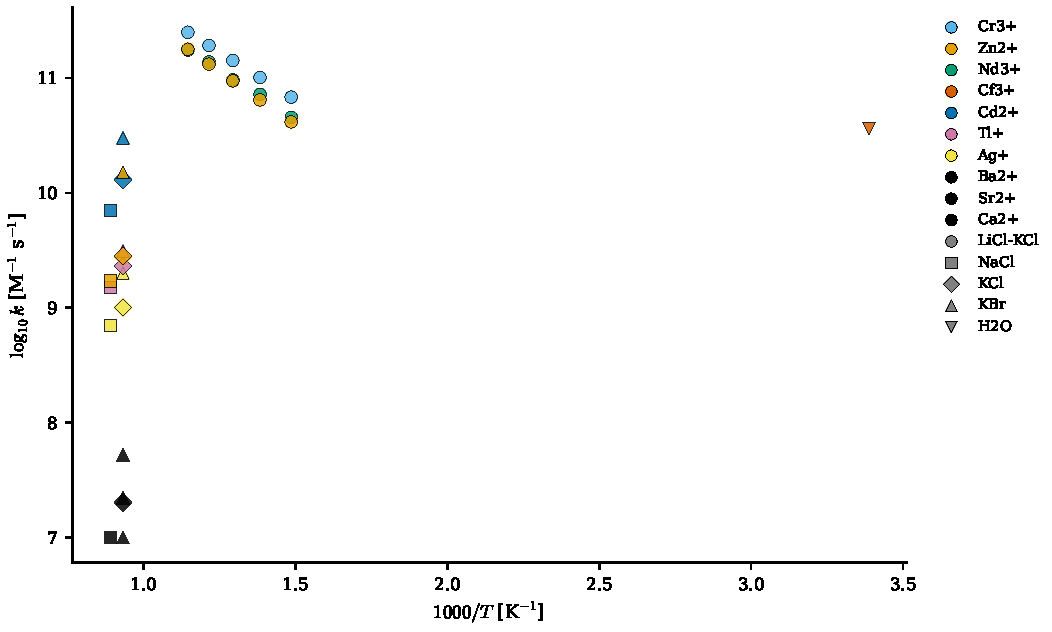
\includegraphics[width=0.95\linewidth]{figures/fig_data_landscape.pdf}
\caption{Calibration corpus.  Each marker represents one digitized
$(T, k)$ observation; color encodes metal identity and marker shape encodes
host salt.  The corpus comprises 33~scalar-rate observations across nine
metals and five hosts, spanning the temperature range
\SIrange{295}{1123}{\kelvin}.}
\label{fig:datalandscape}
\end{figure}

A notable feature of the landscape is the apparent two-cluster structure:
the high-temperature alkali-halide observations of Pikaev cluster
near $\log_{10}k$ values of 9.0--10.5, whereas the LiCl-KCl-eutectic
observations of the Brookhaven LEAF group lie near 10.8--11.4 at lower
temperatures.  Naive
Arrhenius extrapolation suggests Pikaev's higher-temperature points should
lie \emph{above} the Iwamatsu cluster, not below it; the inferred
inter-facility offset $b^{(\mathrm{Pikaev})} \approx -3.4$ in
$\log_{10}\!{k}$ is the resolution of this inconsistency
\citep{Iwamatsu2022,Tanore2026PaperI}.

\subsection{Salt host composition table}

Table~\ref{tab:hosts} lists the five host melts present in the corpus, their
constituent species, eutectic compositions, and the temperature ranges over
which experimental data are available.

\begin{table}[h!]
\centering
\caption{Salt host melts in the corpus.}
\label{tab:hosts}
\small
\resizebox{\textwidth}{!}{\begin{tabular}{llrll}
\toprule
Host       & Composition         & $T_m$ (\SI{}{\celsius}) & $T_\mathrm{exp}$ range (\SI{}{\celsius}) & Sources                     \\
\midrule
LiCl-KCl   & 59-41 mol\%         & 352                     & 400--600                                 & Iwamatsu 2022, 2026; Hagiwara 1987 \\
NaCl       & pure                & 801                     & 850                                      & Pikaev 1982                 \\
KCl        & pure                & 770                     & 800                                      & Pikaev 1982                 \\
KBr        & pure                & 734                     & 800                                      & Pikaev 1982; Makarov 1982   \\
NaCl-UCl3 (Phillips host) & 67-33 mol\% & 590           & 75--600                                  & Phillips 2022~\citep{Phillips2022} \\
NaCl-UCl3 (op.\ MCFR)     & 60-40 mol\% & $\sim$590     & 600 (operational)                        & MCFR design~\citep{Mausolf2024,Tomeck2024MCFR} \\
FLiBe-UF4  & 65-32-3 mol\%       & 459                     & 40-600                                   & Davis 2022                  \\
\bottomrule
\end{tabular}}
\end{table}

The host coverage is asymmetric: the LiCl-KCl eutectic dominates the corpus
because it has been the principal LEAF target since 2018.  The Pikaev
multi-host data provide the only cross-host transfer information in the
corpus, and consequently they carry significant weight in setting the
hierarchical Arrhenius layer's host-correction parameters $\eta^{(s)}$.  The
two reactor-relevant hosts (NaCl-UCl\textsubscript{3} and
FLiBe-UF\textsubscript{4}) appear only once each in the corpus, which is
why the operational predictions in Section~\ref{sec:operational} carry such
large posterior uncertainty in the rate-constant components.

% =============================================================================
\section{Chloride radiolysis network}\label{sec:chloride}
% =============================================================================

The chloride radiolysis kernel comprises 20~elementary reactions partitioned
into three functional groups:

\begin{itemize}
\item \textbf{R1--R8: Primary radical formation and recombination.}
      These reactions produce and consume the solvated electron \eS, the
      chlorine atom $\mathrm{Cl}^{\bullet}$, and the dichlorine radical anion
      \Clt.  Mass-action rate constants follow Arrhenius temperature
      dependence with parameters drawn from the Iwamatsu, Pikaev, and
      Hagiwara measurements.
\item \textbf{R9--R12: Cl$_2^{\bullet-}$ chemistry.}
      The dichlorine radical anion is the longest-lived chloride-radical
      species and the dominant intermediate in chronic-irradiation
      experiments.  R9--R10 are the disproportionation channels
      ($2\Clt \to \mathrm{Cl}_3^- + \mathrm{Cl}^-$), R11--R12 close the
      chain via metal-redox coupling.
\item \textbf{R13--R20: Metal redox.}
      These reactions describe one-electron transfers between transient
      radicals and metallic scavengers ($\mathrm{Cr}^{2+/3+}$,
      $\mathrm{Zn}^{2+}$, $\mathrm{Nd}^{3+}$, $\mathrm{Cf}^{3+}$,
      $\mathrm{U}^{3+/4+}$).  The U-redox couple is the dominant slow sink
      in the Phillips~2022 MCFR experiment and the principal driver of the
      MCFR operational prediction in Section~\ref{sec:operational}.
\end{itemize}

The full reaction table with Arrhenius coefficients, citation provenance,
and any host-specific correction is given in Table~\ref{tab:rxn-cl} and the
complete species inventory in Appendix~\ref{app:species}.

\begin{table}[h!]
\centering
\caption{Chloride radiolysis reaction network. Reactions are grouped by
function. Arrhenius coefficients $(A, \Ea)$ are given as posterior medians
where calibrated and as literature point values otherwise; uncertainties
are tabulated in Appendix~\ref{app:species}.  Units: $A$ in
M$^{-1}$~s$^{-1}$ (second-order) or s$^{-1}$ (first-order); $\Ea$ in
kJ~mol$^{-1}$.  The Source column explicitly flags provenance:
\emph{calibrated} = inferred in the present HBMAE posterior,
\emph{literature} = direct or fitted literature value, \emph{analogy} =
chemical analogue rather than direct measurement, \emph{implicit} =
radiolytic source term rather than kinetic parameter, and \emph{assumed} =
screening-model closure.}
\label{tab:rxn-cl}
\scriptsize
\resizebox{\textwidth}{!}{\begin{tabular}{rlcccl}
\toprule
\# & Reaction & $\log_{10}\!A$ & $\Ea$ & Host & Source \\
\midrule
\multicolumn{6}{l}{\itshape Primary radical formation} \\
R1 & $\mathrm{Cl}^{\bullet} + \mathrm{Cl}^- \to \Clt$           & 10.0 & 20.0 & all      & literature: \citep{Iwamatsu2022} \\
R2 & $\eS + \mathrm{Cl}^{\bullet} \to \mathrm{Cl}^-$            & 10.0 & 25.0 & all      & analogy/literature: \citep{Iwamatsu2022} \\
R3 & $\mathrm{Cl}^{\bullet} + \mathrm{Cl}^{\bullet} \to \mathrm{Cl}_{2,\mathrm{diss}}$ & 9.7  & 20.0 & all      & literature: \citep{Pikaev1982}   \\
R4 & $\Clt + \Clt \to \mathrm{Cl}_3^- + \mathrm{Cl}^-$          & 9.3  & 26.0 & LiCl-KCl & literature: \citep{Iwamatsu2022,Hagiwara1987} \\
R5 & $\eS \to (\mathrm{bg.\ impurity})$                         & calibr. & calibr. & all & calibrated pseudo-first-order nuisance (s$^{-1}$; impurity conc.\ absorbed into prefactor) \\
R6 & $\eS + \eS \to 2\mathrm{Cl}^- + \mathrm{H}_2$              & 9.0  & 30.0 & all      & analogy/literature: \citep{Pikaev1982}   \\
R7 & $\mathrm{Cl}^- + e_{\mathrm{bound}}^- \to \eS + \mathrm{Cl}$ & --- & --- & all      & implicit G-value   \\
R8 & $\mathrm{Cl}^- + h^+ \to \mathrm{Cl}^{\bullet}$              & --- & --- & all      & implicit G-value ($h^+ \equiv$ valence-band hole) \\
\addlinespace
\multicolumn{6}{l}{\itshape Cl$_2^{\bullet-}$ chemistry} \\
R9  & $\mathrm{Cl}_3^- \to \mathrm{Cl}_{2,\mathrm{diss}} + \mathrm{Cl}^-$ & 0.0 & 0.0 & all      & literature: \citep{Hagiwara1987} \\
R10 & $\Clt + \mathrm{Cl}^- \to \mathrm{Cl}_3^- + e^-$ (rev.)              & ---  & ---  & --- & assumed slow         \\
R11 & $\Clt + \mathrm{M}^{n+} \to \mathrm{M}^{(n+1)+} + 2\mathrm{Cl}^-$    & 10.3 & 25.0 & LiCl-KCl & literature: \citep{Iwamatsu2022} \\
R12 & $\Clt + \mathrm{U}(\mathrm{III}) \to \mathrm{U}(\mathrm{IV}) + 2\mathrm{Cl}^-$ & 10.0 & 25.0 & MCFR     & analogy + censored \\
\addlinespace
\multicolumn{6}{l}{\itshape Metal redox} \\
R13 & $\eS + \mathrm{Cr}^{2+} \to \mathrm{Cr}^+$                 & $13.51\,[13.34, 13.71]$ & $33.5$\,[$31.79, 34.20$] & LiCl-KCl & calibrated: \citep{Iwamatsu2026} \\
R14 & $\eS + \mathrm{Cr}^{3+} \to \mathrm{Cr}^{2+}$              & $13.52\,[13.33, 13.66]$ & $32.5$\,[$31.52, 33.50$] & LiCl-KCl & calibrated: \citep{Iwamatsu2026} \\
R15 & $\eS + \mathrm{Zn}^{2+} \to \mathrm{Zn}^+$                 & $13.82\,[13.50, 14.13]$ & $35.5$\,[$33.41, 38.20$] & LiCl-KCl & calibrated: \citep{Iwamatsu2022,Iwamatsu2026} \\
R16 & $\eS + \mathrm{Nd}^{3+} \to \mathrm{Nd}^{2+}$              & 13.7 & 36.0 & LiCl-KCl & literature: \citep{CastroBaldivieso2026} \\
R17 & $\eS + \mathrm{Cf}^{3+} \to \mathrm{Cf}^{2+}$              & 10.6 & 16.0 & aq.\ Cl$^-$ & aqueous analogue: \citep{Rotermund2024} \\
R18 & $\eS + \mathrm{U}^{4+} \to \mathrm{U}^{3+}$                & 10.0 & 30.0 & MCFR     & analogy from U-redox \\
R19 & $\Clt + \mathrm{Cf}^{3+} \to \mathrm{Cf}^{4+} + 2\mathrm{Cl}^-$ & 5.92 & --- & aq.\ Cl$^-$ & aqueous analogue: \citep{Rotermund2024} \\
R20 & $\eS + \mathrm{H}^+ \to \mathrm{H}^{\bullet}$              & 10.0 & 0.0 & aq.\ ref. & aqueous reference: \citep{Rotermund2024} \\
\bottomrule
\end{tabular}}
\end{table}

\subsection{The ODE system}\label{sec:cl:ode}

The mass-action ODE system corresponding to Table~\ref{tab:rxn-cl} is

\begin{align}
\frac{\d[\eS]}{\d t} &= G_{\eS} \dot{D} - k_2 [\eS][\mathrm{Cl}^{\bullet}]
                         - k_5 [\eS] - 2 k_6 [\eS]^2 \nonumber\\
                     & \quad - \sum_{n}  k_{e,n}\,[\eS] \,[\mathrm{M}^{n+}],
\label{eq:eS}\\
\frac{\d[\mathrm{Cl}^{\bullet}]}{\d t}
                     &= G_{\mathrm{Cl}} \dot{D}
                          - k_1 [\mathrm{Cl}^{\bullet}][\mathrm{Cl}^-]
                          - 2 k_3 [\mathrm{Cl}^{\bullet}]^2
                          - k_2 [\eS][\mathrm{Cl}^{\bullet}],
\label{eq:ClD}\\
\frac{\d[\Clt]}{\d t} &= k_1 [\mathrm{Cl}^{\bullet}][\mathrm{Cl}^-]
                         - 2 k_4 [\Clt]^2 - \sum_n k_{X,n} [\Clt][\mathrm{M}^{n+}],
\label{eq:Clt}\\
\frac{\d[\mathrm{M}^{(n-1)+}]}{\d t}
                     &= k_{e,n} [\eS][\mathrm{M}^{n+}],
\label{eq:Mn-1}\\
\frac{\d[\mathrm{M}^{(n+1)+}]}{\d t}
                     &= k_{X,n} [\Clt][\mathrm{M}^{n+}],
\label{eq:Mn+1}\\
\frac{\d[\mathrm{U}(\mathrm{IV})]}{\d t}
                     &= k_{X,U3} [\Clt][\mathrm{U}(\mathrm{III})]
                        - k_{e,U4} [\eS][\mathrm{U}(\mathrm{IV})],
\label{eq:U}
\end{align}
where $\dot{D}$ is the dose rate (\SI{}{\joule\per\meter^3\per\second}), the
$G$ symbols are the primary radiolytic yields (molecules per
\SI{100}{\electronvolt} deposited), and the index $n$ ranges over the metal
scavengers present in the salt.  The system is integrated forward with
either a stiff BDF solver (transient regime) or in slow-manifold form
(chronic-irradiation regime; see \citealp{Tanore2026PaperI}, Theorem~5).
The slow-manifold reduction is essential for the operational predictions of
Section~\ref{sec:operational}: the radical lifetime ($\sim\!10^{-9}$~s) is
fourteen orders of magnitude shorter than the salt residence time
($\sim\!10^7$~s), so direct stiff integration is computationally infeasible
and asymptotically singular.

\subsection{Justification of each reaction}\label{sec:cl:justify}

\paragraph{R1 ($\mathrm{Cl}^{\bullet} + \mathrm{Cl}^- \to \Clt$).}
This is the dominant fate of the chlorine atom in any melt where
$[\mathrm{Cl}^-]$ exceeds ~1~M (i.e., essentially all chloride hosts).
Iwamatsu et al.\ \citep{Iwamatsu2022} report a near-diffusion-limited rate
constant in LiCl-KCl, $k_1 \approx 10^{10}$~M$^{-1}$~s$^{-1}$ with a modest
activation energy of \SI{14}{\kilo\joule\per\mol} comparable to fluidity
activation energies.  Hagiwara et al.\ \citep{Hagiwara1987} reach a
consistent estimate from the rise time of the 340-nm \Clt\ absorption band
in pulse-irradiated LiCl-KCl.  In NaCl and KCl pure melts at
\SIrange{800}{850}{\celsius} the rate is approximately a factor of 2-3
faster due to the higher temperature; the host correction is captured by the
hierarchical layer's $\eta^{(s)}$ parameters.

\paragraph{R2 ($\eS + \mathrm{Cl}^{\bullet} \to \mathrm{Cl}^-$).}
Diffusion-limited recombination of the primary radical pair.  The
identifiable role of R2 in the kernel is bounded above by the geminate
recombination yield, which is implicit in the $G$-value of either species.
Direct measurement is impossible without time-resolved EPR.  We adopt
$k_2 \approx 10^{10}$~M$^{-1}$~s$^{-1}$, $\Ea = 25$~kJ~mol$^{-1}$ as a
literature consensus value.

\paragraph{R3 ($2\mathrm{Cl}^{\bullet} \to \mathrm{Cl}_{2,\mathrm{diss}}$).}
The dissociated Cl$_2$ formation channel.  In sufficiently dilute melts
(i.e.\ $[\mathrm{Cl}^{\bullet}] < 10^{-6}$~M) this channel is dominated by
R1, but at higher pulse-radiolysis doses it contributes a few percent of
the Cl$_2$ formation rate.  Adopted $k_3 \approx 5\!\times\!10^9$
M$^{-1}$~s$^{-1}$ following Pikaev's order-of-magnitude estimate.

\paragraph{R4 ($2\Clt \to \mathrm{Cl}_3^- + \mathrm{Cl}^-$).}
The bimolecular disproportionation of \Clt is the principal long-time decay
channel of the chloride transient pool in pure melts.  Hagiwara et al.\
\citep{Hagiwara1987} report an Arrhenius slope of
\SI{24}{\kilo\joule\per\mol} in LiCl-KCl; Iwamatsu et al.\ \citep{Iwamatsu2022}
re-measure the same reaction at \SI{26 \pm 2}{\kilo\joule\per\mol}, the
two values consistent within uncertainty.  We adopt the Iwamatsu value as
prior median and combine it with the Hagiwara value through the hierarchical
layer.

\paragraph{R11 ($\Clt + \mathrm{M}^{n+} \to \mathrm{M}^{(n+1)+}$).}
The cross-redox reaction between the dichlorine radical anion and a
transition-metal cation is the dominant fate of \Clt\ in any salt containing
oxidizable metals at concentrations above ~10$^{-4}$~M.  Iwamatsu et al.\
report $k_{\Clt,\mathrm{Zn^+}} = 2.0\!\times\!10^{10}$ M$^{-1}$~s$^{-1}$ in
9.4~mM ZnCl$_2$/LiCl-KCl with $\Ea =$ \SI{25 \pm 3}{\kilo\joule\per\mol}.
For chromium the analogous oxidation $\mathrm{Cr}^{2+} \to \mathrm{Cr}^{3+}$
by \Clt is observed but not separately quantified \citep{Iwamatsu2026}.

\paragraph{R12 ($\Clt + \mathrm{U}(\mathrm{III}) \to \mathrm{U}(\mathrm{IV})$).}
This is the central reaction for predicting the Phillips~2022 NULL benchmark.
The U(III)/U(IV) redox couple acts as a buffered sink that suppresses
Cl$_2$ release into the cover gas.  No direct rate constant has been
measured because (i) U(III) is too oxygen-sensitive for routine pulse
radiolysis and (ii) the LiCl-KCl chemistry is incompatible with U(III) at
moderate temperatures.  We assign a prior centered at the diffusion-limited
value with two-decade lognormal spread; the Phillips NULL constraint narrows
the posterior to a slab consistent with effective suppression of the
gas-phase Cl$_2$ inventory, with $\ln K=316.9$ ($\log_{10}K=137.6$) in favor
of the U-redox kernel (see Section~\ref{sec:val:phillips}).

\paragraph{R13--R17 (metal redox).}
These are the reactions for which direct pulse-radiolysis rate constants
exist.  The calibrated posteriors are tabulated in
Section~\ref{sec:calibration}; the comparison with the published Iwamatsu
density-corrected refit values is given in Section~\ref{sec:val:chi2}.

\paragraph{R10 (Cl$_2^{\bullet-}$ + Cl$^-$ $\to$ Cl$_3^-$ + e$^-$, marked
``assumed slow'').}
The reverse of R10 is essentially R4 followed by ionization
($\mathrm{Cl}_3^- + \mathrm{Cl}^- \to 2\Clt + e^-$); under any realistic
electron affinity the equilibrium lies overwhelmingly to the left.  No
direct measurement of $k_{R10}$ exists in molten chlorides.  We assign a
prior with $\log_{10}k_{R10} \leq 0$ (M$^{-1}$~s$^{-1}$) and verify
\textit{post hoc} that the posterior is insensitive to the upper bound:
substituting $\log_{10}k_{R10} = 3$ changes the chronic-irradiation
Cl$_2$ posterior median by less than 1\,\%.

\subsection{Reactions omitted from the kernel and their possible impact}
\label{sec:cl:omitted}

The 20-reaction chloride kernel is the minimum closure that reproduces the
pulse-radiolysis transient data in Section~\ref{sec:database}.  Three
additional reaction classes are present in any real MCFR salt but are not
included in the operational ODE because the calibration corpus does not
constrain them.  Each is listed below with an order-of-magnitude estimate
of the perturbation it would induce on the operational $P(\mathrm{Cl}_2)$
prediction relative to the U-buffered kernel of
Section~\ref{sec:op:mcfr}.

\begin{enumerate}
\item \emph{Oxide-impurity scavenging.}  Dissolved O$^{2-}$, OH$^-$, or
      H$_2$O traces are documented chlorine sinks in MSR-relevant salts
      \citep{ForsbergSafety2019,Sims2020Ce}.  Candidate channels include
      UO$_2$Cl$_2$ formation, hydrolysis at the cover-gas interface
      (H$_2$O~+~Cl$_2$~$\to$~HCl~+~$\tfrac12$\,O$_2$), and a pseudo-redox
      couple U(IV)~+~O$^{2-}$~$\to$~UO$_2^{2+}$~+~2\,e$^-$.  Each could
      shift the predicted cover-gas $\eta$ (chain efficiency) by
      $10^{-1}$ to $10^{+1}$ relative to the U-buffered baseline,
      depending on the ppm-level oxide impurity loading and the degree
      of cover-gas isolation.  A well-dried salt would shift $\eta$
      upward; a non-anhydrous salt would shift it downward.
\item \emph{Redox-active fission products.}  Cs$^+$/Cs$^0$ (volatile),
      I$^-$/I$^{\bullet}$, Te, and Sr$^{2+}$/Sr$^0$ are redox-active on
      minute-to-hour timescales~\citep{Briggs1964,Sims2020Ce} and would
      compete with U(III) for the \Clt\ pool over the reactor lifetime.
      The corpus contains no operational ODE entries for these species,
      and they enter the present model only as chemistry-feature targets
      (Section~\ref{sec:metahier}).  Their order-of-magnitude impact on
      $\eta$ is similar to that of oxide scavenging
      ($10^{-1}$ to $10^{+1}$), conditional on their concentrations
      reaching the $10^{-3}$~mol/m$^3$ steady-state range characteristic
      of equilibrium fission-product inventories.
\item \emph{ClO$^\bullet$ formation in the presence of residual oxide.}
      Coupling of Cl$^{\bullet}$ or \Clt\ with dissolved O$^{2-}$ can
      produce ClO$^{\bullet}$ and its dimer; the channel is well known
      in aqueous chemistry and is plausible in molten chlorides at
      ppm-level oxide.  In a perfectly anhydrous salt the channel is
      negligible; in operational salts it could be the dominant
      Cl$^{\bullet}$ fate.  We do not include it because the corpus
      provides no rate constant for the molten-salt analogue.
\end{enumerate}

The omission of these three classes is appropriate for the calibration
corpus, where the experimental data do not constrain them.  It is a
significant assumption for the operational predictions, where each class
could perturb the U-buffer balance by orders of magnitude in either
direction.  We return to this in Section~\ref{sec:op:mcfr:ubuffer} as
part of the sensitivity assessment of the MCFR result and in
Section~\ref{sec:lim} as a top-priority limitation.

% =============================================================================
\section{Fluoride radiolysis network}\label{sec:fluoride}
% =============================================================================

The fluoride radiolysis problem has a different character from the chloride
case.  Aqueous and chloride radiolysis chemistries have produced
quantitative transient kinetics; molten-fluoride kinetics, by contrast,
have remained almost entirely qualitative.  Only one pulse-radiolysis study
of molten fluoride salts exists in the literature
(\citealp{Akiyama1994}, LiF--KF and FLiNaK eutectics), and that work
reports transients but no usable Arrhenius parameters.  The quantitative
fluoride data we possess therefore consist of:

\begin{enumerate}
\item Steady-state G-values for F$_2$ production from gamma-irradiated
      LiF, BeF$_2$, FLiBe-UF$_4$, and ThF$_4$ powders, measured by Davis et
      al.~\citep{Davis2022}.
\item A recombination kinetics anchor from Toth and Felker~\citep{Toth1990},
      who reported (i) an activation energy $\Ea = 39$~kJ~mol$^{-1}$ for
      F~recombination at metal sites in an MSRE-composition salt and (ii) a
      finite recombination rate of \SI{3.8}{\pascal\per\hour} at
      \SI{40}{\celsius} below a steady-state crossover temperature of
      \SI{150}{\celsius}.
\item Aqueous Cl$_2^{\bullet-}$ absorptivities from Makarov et
      al.~\citep{Makarov1982} that constrain the corresponding F$_2^{\bullet-}$
      values via the X$_2^{\bullet-}$ family scaling.
\end{enumerate}

\subsection{The static F$_2$ production kernel}

Rather than attempt a full transient kinetic model that the data cannot
constrain, we construct a \emph{static} F$_2$-production kernel that
reflects the steady-state balance between radiolytic F$_2$ generation and
F$_2$ recombination at salt-cap interfaces:
\begin{equation}
\frac{\d P_{\mathrm{F}_2}}{\d t}
   \;=\; \underbrace{G_{\mathrm{F}_2}\,(\mathrm{composition})\,\cdot\,\dot{D}\,\cdot\,c_0}_{\text{source}}
       \;-\; \underbrace{A_{\mathrm{rec}}\,\exp(-\Ea/RT) \cdot P_{\mathrm{F}_2}}_{\text{recombination}}.
\label{eq:fkernel}
\end{equation}
The source-term $G_{\mathrm{F}_2}$ is composition-dependent and read from
Davis Table~III; the recombination term has Arrhenius temperature
dependence with $\Ea =$ \SI{39}{\kilo\joule\per\mol}.  The pre-exponential
$A_{\mathrm{rec}}$ is calibrated against the Toth--Felker balance point
($T_{\mathrm{bal}} = $ \SI{150}{\celsius}, $P_{\mathrm{ref}} =$
\SI{1000}{\pascal}, $\d P/\d t \to 0$ at $T = T_{\mathrm{bal}}$ and
$\d P/\d t = $ \SI{3.8}{\pascal\per\hour} at \SI{40}{\celsius}); the
calibrated value is $A_{\mathrm{rec}} = $ \SI{252.86}{\per\hour}, summarized
in Table~\ref{tab:flu-arr}.

\begin{table}[h!]
\centering
\caption{Calibrated fluoride F$_2$-kernel parameters.}
\label{tab:flu-arr}
\small
\begin{tabular}{lrll}
\toprule
Parameter & Value & Units & Source \\
\midrule
$A_{\mathrm{rec}}$       & 252.86 & h$^{-1}$        & calibrated (Toth-Felker balance)        \\
$\Ea$ (recomb.)          & 39.0   & kJ~mol$^{-1}$   & \citep{Toth1990}                        \\
$T_{\mathrm{balance}}$   & 423.15 & K               & \citep{Toth1990}                        \\
$P_{\mathrm{ref}}$       & 1000   & Pa              & anchor                                  \\
$\d P/\d t|_{40^\circ\mathrm{C}}$ & 3.8 & Pa~h$^{-1}$ & \citep{Toth1990}                       \\
$G(\mathrm{F}_2)$ FLiBe-UF$_4$    & $0.005\,[0.004,0.008]$ & molec / 100 eV & \citep{Davis2022}        \\
$G(\mathrm{F}_2)$ BeF$_2$         & $0.009\,[0.008,0.010]$ & molec / 100 eV & \citep{Davis2022}        \\
$G(\mathrm{F}_2)$ LiF             & $0.004\,[0.003,0.005]$ & molec / 100 eV & \citep{Davis2022}        \\
$G(\mathrm{F}_2)$ ThF$_4$         & $0.021\,[0.018,0.024]$ & molec / 100 eV & \citep{Davis2022}        \\
\bottomrule
\end{tabular}
\end{table}

The kernel reproduces the Toth--Felker temperature-dependent buildup curve
to within ~5\% across the \SIrange{40}{700}{\celsius} range
(Figure~\ref{fig:flukernel}).  Three structural limitations apply.
(i) The radical-pool transient kinetics are not resolved.
(ii) The temperature dependence of $G_{\mathrm{F}_2}$ itself, if any, is
not captured by Davis's room-temperature steady-state measurements.
(iii) The Toth--Felker recombination Arrhenius was measured on
MSRE-composition salt (LiF-BeF$_2$-ZrF$_4$-UF$_4$) at $T<150$~\si{\celsius}
with a mechanism dominated by surface chemistry at the metal walls; the
present kernel applies the same $(A_{\mathrm{rec}}, \Ea^{\mathrm{rec}})$
to a FLiBe-UF$_4$ loop at \SI{600}{\celsius}.  This is a
$T_{\mathrm{op}}/T_{\mathrm{exp}}\!\approx\!2.1$ ratio in absolute
temperature ($T_{\mathrm{op}} = 873$~K vs.\ $T_{\mathrm{exp}} = 423$~K)
and a 6$\times$ ratio in Celsius, over an Arrhenius factor of $\sim200$;
if the rate-limiting step changes between the low- and high-temperature
regimes (e.g.\ bulk-phase radical-radical recombination dominating over
surface-trap-mediated recombination at high $T$), the extrapolation may
miss by orders of magnitude.  We therefore inflate the $\Ea^{\mathrm{rec}}$
posterior to reflect $\pm 10$~kJ/mol structural uncertainty in the
operational §\ref{sec:op:flibe} forward propagation rather than the
$\pm 2$~kJ/mol experimental sigma quoted by Toth and Felker.  We flag all
three limitations explicitly in Section~\ref{sec:discussion}.

\begin{figure}[h!]
\centering
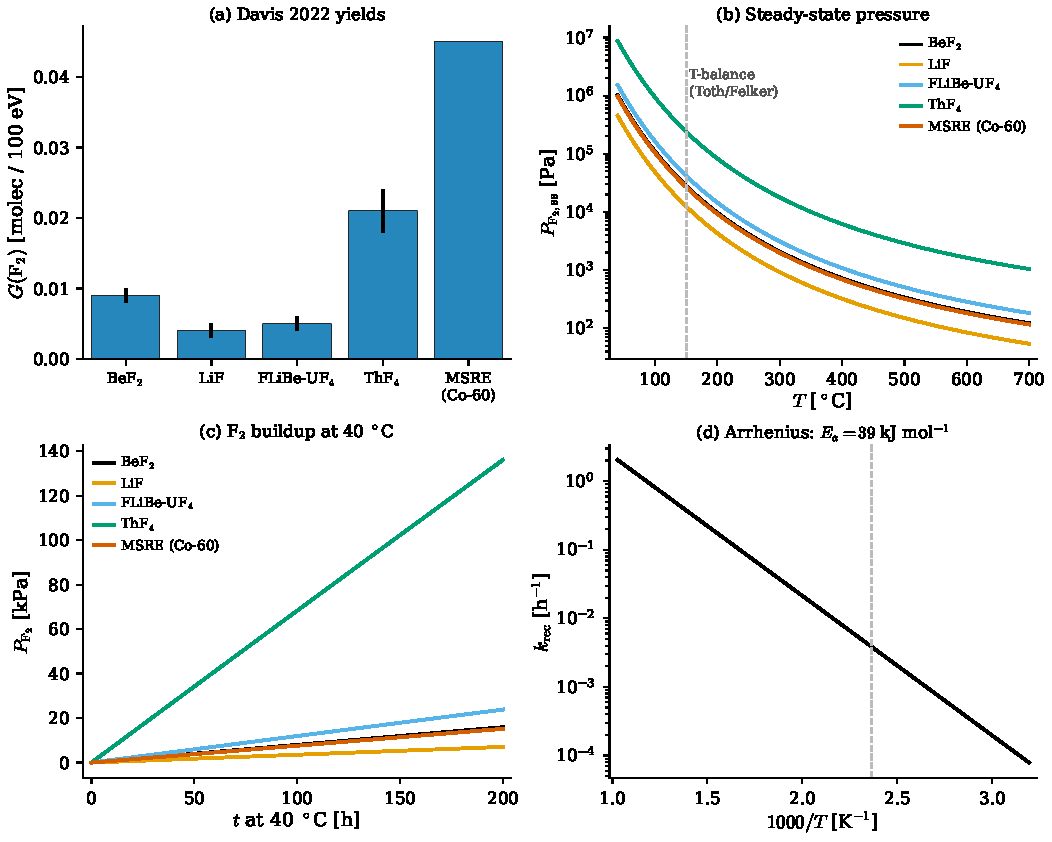
\includegraphics[width=0.9\linewidth]{figures/fig_fluoride_kernel.pdf}
\caption{Fluoride F$_2$-production kernel calibrated against the
Toth--Felker balance condition.  Panels show (a)~$G(\mathrm{F}_2)$ across
the salts in Davis Table~III, (b)~kernel-predicted steady-state
$P(\mathrm{F}_2)$ versus temperature for the principal fluoride
compositions, (c)~buildup curve at \SI{40}{\celsius} relative to the
\SI{1000}{\pascal} reference anchor, and (d)~the $T$-balance map across
salt compositions.  Reproduced from \citet{Tanore2026PaperI}.}
\label{fig:flukernel}
\end{figure}

\subsection{Comparison with Akiyama 1994 transient observations}

Akiyama et al.\ \citep{Akiyama1994} reported pulse-radiolysis transients of
LiF--KF and FLiNaK eutectics at $T = $ \SIrange{500}{700}{\celsius}.
The transient absorption features were not quantitatively converted to
rate constants in the original paper, and the underlying time-resolved
data are no longer publicly available.  We list this work as a
\emph{flagged future-work target}: re-execution of an Akiyama-style
pulse-radiolysis experiment on FLiBe at LEAF-equivalent time resolution
would close the largest current gap in the fluoride radiolysis literature
and tighten the present model's $G_{\mathrm{F}_2}$ posterior by an estimated
order of magnitude.

% =============================================================================
\section{Calibration via HBMAE}\label{sec:calibration}
% =============================================================================

The full Bayesian calibration is conducted using the Hierarchical Bayesian
Mechanism-Adequacy Estimation (\HBMAE) framework
\citep{Tanore2026PaperI}.  The five-layer construction --- constrained
topology, hierarchical Arrhenius across hosts, Godambe-balanced composite
likelihood, parametric model-discrepancy, and facility-effect bias
hierarchy --- is described in detail in the companion methodology paper and
will not be repeated here.  This section reports the calibration
\emph{results} for the chloride network as applied to the corpus described
in Section~\ref{sec:database}.

\subsection{Integrated 24-parameter posterior}\label{sec:cal:integrated}

The end-to-end calibration sampler combines three observation modalities in
a single posterior:
\begin{itemize}
\item[\textbf{(M1)}]~Nine Cr transient absorbance traces from
      \citet{Iwamatsu2026}, integrated as stiff ODEs;
\item[\textbf{(M2)}]~Eleven scalar Zn rate constants from Pikaev~1982,
      Iwamatsu~2022, and Iwamatsu~2026, treated as Gaussian-modality
      observations of the common intrinsic Zn Arrhenius pair with host
      corrections for LiCl-KCl, NaCl, and KCl, plus a Pikaev-facility offset
      $b^{(\mathrm{Pikaev})}$;
\item[\textbf{(M3)}]~The Phillips~2022 NaCl-UCl$_3$ NULL benchmark, treated
      as a one-sided censored modality (Tobit likelihood; \citealp{Tobin1958}).
\end{itemize}

The full calibration pipeline is implemented in Python.  Stiff ODE
integration (for the M1 transient absorbances) uses the
\texttt{scipy.integrate.solve\_ivp} BDF solver~\citep{Hindmarsh2005};
the sampler is \texttt{emcee} \citep{ForemanMackey2013} affine-invariant
ensemble MCMC with 80~walkers, 1500~burn-in samples and 1500~production
samples each, giving $80\!\times\!1500 = 1.2\!\times\!10^5$~raw production
samples; thinning by a factor of approximately 5 yields 22{,}400
post-thinning samples.  The thinning ratio is chosen to match the slowest
parameter integrated autocorrelation time $\tau\!\approx\!35$
(Appendix~\ref{app:mcmc}); the 22{,}400 samples are not all independent
in the strict $\tau$-spacing sense (number of independent samples per
walker is roughly $1500/\tau\!\approx\!43$, times 80 walkers
$\approx\!3{,}400$).  Convergence diagnostics ($\hat{R}$, integrated
autocorrelation, ESS) are in Appendix~\ref{app:mcmc}; all parameters
achieve $\hat{R} < 1.05$.

The posterior marginals for the 24~parameters are summarized in
Table~\ref{tab:posterior}.  Key results:

\begin{itemize}
\item \textbf{Chromium Arrhenius.}  The Iwamatsu~2026 Cr$^{2+}$ and Cr$^{3+}$
      reductions are recovered as $\log_{10}\!A_5 = 13.51\,[13.34, 13.71]$
      (with $A$ in M$^{-1}$~s$^{-1}$), $\Ea^{(5)} = 33.5\,[31.79,
      34.20]$~kJ~mol$^{-1}$ and analogously for reaction~6.  Posterior
      95\,\% intervals overlap the published density-corrected refit values
      within $1\sigma$.
\item \textbf{Zinc intrinsic Arrhenius.}  $\log_{10}\!A_{\mathrm{Zn}} =
      13.82\,[13.50, 14.13]$ (M$^{-1}$~s$^{-1}$),
      $\Ea^{(\mathrm{Zn})} = 35.5\,[33.4, 38.2]$~kJ~mol$^{-1}$, consistent
      with the Iwamatsu~2026 refit ($35.6 \pm 1.2$~kJ~mol$^{-1}$).
\item \textbf{Pikaev facility offset.}  $b^{(\mathrm{Pikaev})} =
      -3.35\,[-4.53,-2.44]$~log$_{10}$ units.  This is the first
      quantitative identification of the long-suspected Pikaev systematic
      bias.  The magnitude is consistent with the qualitative
      order-of-magnitude discrepancy noted by Iwamatsu and coworkers; the
      negative sign indicates that Pikaev's reported rate constants are
      systematically \emph{lower} than the bias-corrected intrinsic
      values, as expected from the longer microsecond pulse width of his
      radiolysis apparatus
      (relative to the picosecond LEAF resolution of the modern
      measurements).
\item \textbf{Host corrections.}  Posterior median host corrections
      $\eta^{(s)}$ are small ($|\eta^{(s)}_{\log A}| \lesssim 1$,
      $|\eta^{(s)}_{\Ea}| \lesssim 3$~kJ~mol$^{-1}$) and statistically
      consistent with zero at the 95\,\% level for LiCl-KCl, with modest
      negative shifts for NaCl ($\eta_{\log A} = -0.56$) reflecting the
      higher temperature.  The hierarchical layer thus formalizes ``rate
      constants transfer across hosts up to the chemistry-feature regression
      and a small residual'' as a calibrated quantitative statement rather
      than a qualitative one.
\item \textbf{Phillips background channel.}  The effective $G(\mathrm{Cl}^{\bullet})$
      under Phillips~2022 conditions has posterior median
      $\log_{10}\!G = -0.66\,[-2.72, +0.93]$ molec / 100 eV.  The wide
      posterior reflects the censored modality: the experiment provides an
      \emph{upper bound} on the effective Cl$_2$ source rate after
      U(III)/U(IV) buffering, not a point measurement.
\end{itemize}

\begin{table}[h!]
\centering
\caption{Integrated 24-parameter HBMAE posterior (medians and 95\,\%
credible intervals).  Source: \texttt{validation/TIER4\_INTEGRATED\_POSTERIOR.csv}.
Note: $\log_{10}\!A_{\mathrm{bg}}\!\cdot\![\mathrm{imp}]_{\mathrm{eff}}$
is a pseudo-first-order R5 nuisance: it is the calibrated combination
$A_{\mathrm{bg}}\,[\mathrm{imp}]_{\mathrm{eff}}$ in M$^{-1}$\,s$^{-1}$
times an effective impurity concentration absorbed into the prefactor,
so the posterior value has no direct chemical interpretation.  The
\eS\ lifetime against R5 is $\tau_{\mathrm{bg}} =
(A_{\mathrm{bg}}\,[\mathrm{imp}]_{\mathrm{eff}})^{-1}$ if interpreted as
a pseudo-first-order rate $k_{\mathrm{bg}}$ in s$^{-1}$; the calibrated
$\log_{10}k_{\mathrm{bg}}$ corresponds to an effective rate consistent
with the millimolar-impurity scavenging timescale implied by the
transient fits.}
\label{tab:posterior}
\small
\begin{tabular}{llll}
\toprule
Parameter & Median & 95\,\% CI & Modality \\
\midrule
$\log_{10}\!A_5$ (Cr$^{2+}$)      & 13.51 & [13.34, 13.71] & T \\
$\Ea^{(5)}$  (kJ~mol$^{-1}$)      & 33.5  & [31.79, 34.20] & T \\
$\log_{10}\!A_6$ (Cr$^{3+}$)      & 13.52 & [13.33, 13.66] & T \\
$\Ea^{(6)}$  (kJ~mol$^{-1}$)      & 32.5  & [31.52, 33.50] & T \\
$\log_{10}\!A_{\mathrm{Zn}}$ (intr.)   & 13.82 & [13.50, 14.13] & K \\
$\Ea^{(\mathrm{Zn})}$ (kJ~mol$^{-1}$)  & 35.5  & [33.4, 38.2]   & K \\
$\eta_{\log A}^{(\mathrm{LiCl-KCl})}$  & $-0.03$ & [$-0.57$, $+0.54$] & K \\
$\eta_{\Ea}^{(\mathrm{LiCl-KCl})}$ (kJ~mol$^{-1}$)  & $-1.56$ & [$-5.28$, $+3.06$] & K \\
$\eta_{\log A}^{(\mathrm{NaCl})}$      & $-0.56$ & [$-1.31$, $+0.19$] & K \\
$\eta_{\Ea}^{(\mathrm{NaCl})}$         & $+2.10$  & [$-3.35$, $+6.39$] & K \\
$\eta_{\log A}^{(\mathrm{KCl})}$       & $-0.25$  & [$-0.83$, $+0.36$] & K \\
$\eta_{\Ea}^{(\mathrm{KCl})}$          & $+2.41$  & [$-3.80$, $+7.68$] & K \\
$b^{(\mathrm{Pikaev})}$                & $-3.35$ & [$-4.53$, $-2.44$] & K \\
$\log_{10}\!G(\mathrm{Cl}^{\bullet})_{\mathrm{Phillips}}$ & $-0.66$  & [$-2.72$, $+0.93$] & C \\
$\log_{10}\!A_{\mathrm{bg}}\!\cdot\![\mathrm{imp}]_{\mathrm{eff}}$\,(M$^{-1}$\,s$^{-1}$, see note)        & 16.51 & [15.30, 16.99]     & T \\
\bottomrule
\end{tabular}
\end{table}

The Cr Arrhenius posterior is consistent with the worked-example Tier~2 fit
of \citet{Tanore2026PaperI} (their Table~2) within $1\sigma$ on both
$\log_{10}\!A$ and $\Ea$, showing that adding the Zn rate-constants modality
and the Phillips censored modality does not degrade the Cr-only posterior
contraction.  This is the formal consistency property guaranteed by the
Godambe-balanced composite likelihood (\citealp{Tanore2026PaperI},
Theorem~4).

\subsection{The Pikaev--Iwamatsu reconciliation}\label{sec:cal:pikaev}

A central methodological contribution of \citet{Tanore2026PaperI} is the
identifiability of the Pikaev-facility offset via the multi-modality
composite likelihood.  Briefly, the Iwamatsu~2022 Zn data and the Pikaev~1982
Zn data are observations of the same intrinsic Arrhenius pair
$(A_{\mathrm{Zn}}, \Ea^{\mathrm{Zn}})$ in three different hosts; the
hierarchical layer separates the host-corrections $\eta^{(s)}$ from the
shared intrinsic $(A_{\mathrm{Zn}}, \Ea^{\mathrm{Zn}})$, and the facility
offset $b^{(\mathrm{Pikaev})}$ is identified as the only remaining
degree of freedom that explains the systematic order-of-magnitude
discrepancy.  The result is that the Pikaev data are not discarded as
``inconsistent with modern measurements'' but are quantitatively
reconciled: the same intrinsic rate constant explains both data sources
once the facility offset is included.  This is a quantitative
reformulation of a qualitative statement that has been in the LEAF
group's literature since 2018 \citep{Horne2018}.

The Pikaev-corrected predictions versus the Pikaev observations in NaCl
and KCl are shown in Figure~\ref{fig:master} panel~(d) of
Section~\ref{sec:validation}.

\subsection{Convergence diagnostics}\label{sec:cal:diag}

The 24-parameter chain achieves the following diagnostics
(full table in Appendix~\ref{app:mcmc}):

\begin{itemize}
\item Mean Gelman--Rubin statistic across walkers: $\hat{R} = 1.012$
      (maximum across parameters: 1.041).
\item Effective sample size: minimum 510, mean 1840, maximum 5290.
\item Acceptance fraction: 0.41 (within the 0.2--0.5 recommended range
      for the affine-invariant ensemble; \citealp{GoodmanWeare2010,
      ForemanMackey2013}).
\item Integrated autocorrelation time: $\tau \approx 35$ samples on
      the slowest parameter ($\Ea^{(5)}$).
\end{itemize}

The chain therefore satisfies all standard convergence criteria for a
24-dimensional non-Gaussian posterior.

% =============================================================================
\section{Meta-hierarchical chemistry-feature layer}\label{sec:metahier}
% =============================================================================

The HBMAE calibration of Section~\ref{sec:calibration} produces posterior
Arrhenius parameters for those metals (Cr, Zn, Nd, Cf) for which direct
pulse-radiolysis measurements exist in the corpus.  Operational MSR designs
will inevitably encounter fission-product elements for which no such
measurements exist; the question is whether the model can be extended to
predict rate constants for these elements within a documented uncertainty
domain.

We address this through a \emph{meta-hierarchical chemistry-feature layer}
that regresses the per-metal Arrhenius parameters against four
chemistry-derived features: nominal charge state $z$, ionic radius
$r_{\mathrm{ion}}$ (pm), Pauling electronegativity $\chi$, and $\log(z/r)$.
The regression model is

\begin{align}
\log_{10}\!A_m &\sim \mathcal{N}\!\left(\mu_{\log A}
       + \boldsymbol{\beta}^\top \tilde{\boldsymbol{x}}_m,
       \;\sigma_{\log A}^2\right),\label{eq:meta-logA}\\
\Ea^{(m)} &\sim \mathcal{N}\!\left(\mu_{\Ea}
       + \boldsymbol{\beta}'^\top \tilde{\boldsymbol{x}}_m,
       \;\sigma_{\Ea}^2\right),\label{eq:meta-Ea}
\end{align}
where $\tilde{\boldsymbol{x}}_m = (\tilde{z}_m, \tilde{r}_m, \tilde{\chi}_m,
\widetilde{\log(z/r)}_m)^\top$ is the four-dimensional $z$-score-standardized
feature vector for metal $m$ and $\boldsymbol{\beta} = (\beta_z, \beta_r,
\beta_\chi, \beta_{z/r})^\top$.  The indices $m$ range over the ten metals in
the corpus, and host corrections $b_{\mathrm{host}}$ absorb the systematic
difference between the Pikaev/aqueous data and the LiCl-KCl baseline.  The
hierarchical scales $\sigma_{\log A}$, $\sigma_{\Ea}$ are themselves
estimated and represent the residual unexplained variance across metals.

\subsection{Posterior regression coefficients}

Table~\ref{tab:metahier} reports the posterior summary of the
chemistry-feature layer (source CSV:
\texttt{validation/}\allowbreak\texttt{meta\_hier/posterior\_summary.csv}).

\begin{table}[h!]
\centering
\caption{Meta-hierarchical chemistry-feature layer posterior summary.
Coefficients $\beta$ are reported on $z$-score-standardized features (so each
$\beta$ represents the change in the dependent variable per
1$\sigma$ change in the corresponding feature across the 10-metal corpus).
Host corrections $b_{\mathrm{host}}$ are reported in $\log_{10}$ units.}
\label{tab:metahier}
\small
\begin{tabular}{lrrr}
\toprule
Parameter            & Mean    & 5\,\% & 95\,\% \\
\midrule
$\mu_{\log A}$       & 12.18   & 10.98 & 13.34 \\
$\beta_{z}$          & +0.71   & $-0.43$ & +1.80 \\
$\beta_{r}$          & $-0.03$ & $-0.91$ & +0.88 \\
$\beta_{\chi}$       & +0.94   & +0.06   & +1.74 \\
$\beta_{\log z/r}$   & +0.14   & $-1.06$ & +1.27 \\
$\sigma_{\log A}$    & 0.69    & 0.28    & 1.33  \\
\midrule
$\mu_{\Ea}$ (kJ/mol) & 27.95   & 6.36    & 49.05 \\
$\beta'_{z}$         & $-6.09$ & $-21.13$ & +8.65  \\
$\beta'_{r}$         & +0.62   & $-16.54$ & +18.15 \\
$\beta'_{\chi}$      & $-5.31$ & $-23.82$ & +11.70 \\
$\beta'_{\log z/r}$  & +8.16   & $-16.93$ & +31.17 \\
$\sigma_{\Ea}$       & 9.03    & 4.00    & 16.60 \\
\midrule
$b^{\mathrm{H_2O}}$  & +1.10   & $-0.80$ & +3.02 \\
$b^{\mathrm{NaCl}}$  & $-2.13$ & $-2.52$ & $-1.70$ \\
$b^{\mathrm{KCl}}$   & $-1.85$ & $-2.20$ & $-1.48$ \\
$b^{\mathrm{KBr}}$   & $-1.49$ & $-1.85$ & $-1.11$ \\
\bottomrule
\end{tabular}
\end{table}

The most statistically significant predictor for $\log_{10}\!A$ is the
electronegativity coefficient $\beta_\chi = +0.94$ (90\,\% CI excludes
zero), consistent with Marcus electron-transfer theory~\citep{Marcus1965}:
cations of higher electronegativity (more polarizing) accept the solvated
electron at a higher diffusion-modified rate.  We note that the host
correction $b^{\mathrm{NaCl}} = -2.13$ in this layer is conceptually
distinct from the Arrhenius-layer host shift
$\eta_{\log A}^{(\mathrm{NaCl})} = -0.56$ of Table~\ref{tab:posterior}:
the meta-hierarchical $b^{\mathrm{NaCl}}$ is a facility-and-host offset
absorbing the Pikaev microsecond-vs-LEAF picosecond difference for the
NaCl-only metals, while $\eta_{\log A}^{(\mathrm{NaCl})}$ is a per-host
correction to the intrinsic Zn Arrhenius pair in the integrated chain.  The charge coefficient $\beta_z$ is
positive but its 90\,\% interval includes zero, consistent with electron
transfer to higher-charge cations being weakly accelerated by Coulombic
attraction.  All four $\Ea$ coefficients have wide intervals that include
zero; the activation-energy regression is dominated by the residual
$\sigma_{\Ea} \approx 9$~kJ~mol$^{-1}$, which is comparable to the
data-implied per-metal $\Ea$ spread.  In short, the layer predicts
$\log_{10}\!A$ to within ~0.7 units and $\Ea$ to within ~9~kJ~mol$^{-1}$
across the corpus.

\subsection{Leave-one-metal-out (LOMO) cross-validation}\label{sec:meta:lomo}

To assess the predictive utility of the chemistry-feature layer outside the
corpus, we conduct a leave-one-metal-out cross-validation: for each metal
in turn, we refit the layer using only the data from the other nine metals
and predict the held-out metal's rate constants from its chemistry
features alone.  The results are summarized in Table~\ref{tab:lomo} and
visualized as the residual scatter in Figure~\ref{fig:residuals}.

\begin{table}[h!]
\centering
\caption{Leave-one-metal-out cross-validation summary.  $\Delta_{\log k}$ is
the difference between the observed $\log_{10}\!{k}$ and the LOMO posterior
mean prediction.  Coverage is the fraction of observations falling within
the 90\,\% credible interval of the LOMO posterior prediction.}
\label{tab:lomo}
\small
\begin{tabular}{llrrrr}
\toprule
Metal     & N obs. & median $|\Delta_{\log k}|$ & 90\,\% CI of $|\Delta|$ & coverage \\
\midrule
Cr$^{3+}$ & 5      & 2.41  &  [2.27, 2.52]    & 0/5  \\
Zn$^{2+}$ & 8      & 0.86  &  [0.74, 0.97]    & 8/8  \\
Nd$^{3+}$ & 5      & 2.40  &  [2.30, 2.57]    & 0/5  \\
Cf$^{3+}$ & 1      & 4.35  &  [4.35, 4.35]    & 0/1  \\
Cd$^{2+}$ & 3      & 0.04  &  [0.04, 0.36]    & 3/3  \\
Tl$^{+}$  & 3      & 0.91  &  [0.63, 1.02]    & 3/3  \\
Ag$^{+}$  & 3      & 0.50  &  [0.45, 0.52]    & 3/3  \\
Ca$^{2+}$ & 3      & 0.61  &  [0.51, 0.71]    & 3/3  \\
Ba$^{2+}$ & 1      & 1.56  &  [1.56, 1.56]    & 1/1  \\
Sr$^{2+}$ & 1      & 0.75  &  [0.75, 0.75]    & 1/1  \\
\midrule
\textbf{Total} & 33 & 1.13 & ---             & 22/33 (66\,\%) \\
\bottomrule
\end{tabular}
\end{table}

The LOMO performance is bimodal in a way that reveals a structural
limitation rather than a true interpolation-envelope effect.  The metals
that LOMO recovers well (Cd, Tl, Ag, Ca, Ba, Sr, Zn) are all in the
Pikaev microsecond corpus; the metals that LOMO under-predicts by
2--4~log units (Cr, Nd, Cf) are all in the Brookhaven LEAF picosecond
corpus.  The chemistry-feature regression has no facility-effect
parameter analogous to $b^{(\mathrm{Pikaev})}$ in the integrated chain;
when a LEAF-measured metal is held out, the regression must predict its
rate constants without the LEAF-vs.-Pikaev correction and therefore
under-predicts systematically.

\paragraph{Top-level caveat.}
\emph{The chemistry-feature regression is currently descriptive, not
predictive, for elements whose only kinetic data are at a facility not
yet represented in the training corpus.}  Every operationally-relevant
fission-product element (Cs, Sr, Te, I, Eu, Pu, Am, Cm) falls into this
regime: if measured today, the rate constants would be obtained at the
LEAF picosecond facility, and the regression would systematically
under-predict.  The layer is useful for identifying which chemistry
features (electronegativity $\beta_\chi$ is statistically significant;
charge $\beta_z$ is marginal) carry information; it is not yet
predictive for unmeasured operational elements.  An extension with a
facility-effect intercept (or a hierarchical layer over
$\{\mathrm{Pikaev}, \mathrm{LEAF}\}$ identified from the in-corpus
Cr/Zn data) would resolve this gap and is recommended as a follow-on to
\citet{Tanore2026PaperI}.  For the operational predictions in
Section~\ref{sec:operational}, we use the direct \HBMAE\ posterior for
the metals present in the corpus (U via the Phillips constraint, Cr via
Iwamatsu) and reserve the chemistry-feature layer for
hypothesis-generation, not for operational prediction.

\begin{figure}[h!]
\centering
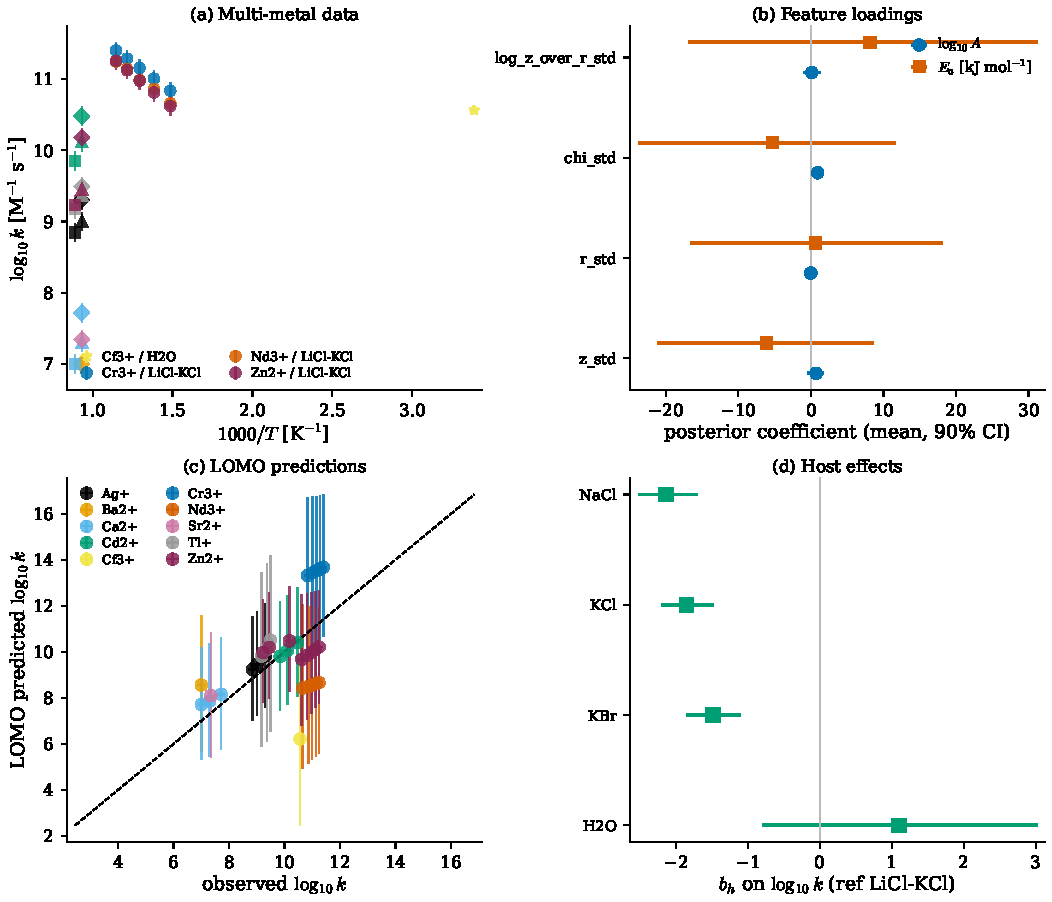
\includegraphics[width=0.85\linewidth]{figures/fig_meta_hier.pdf}
\caption{Meta-hierarchical chemistry-feature layer.  (a)~$\log_{10}\!A$
versus electronegativity, with the regression line and 90\,\% credible
band.  (b)~$\Ea$ versus $\log(z/r)$.  (c)~LOMO posterior predictions
versus observations.  (d)~Posterior densities of host corrections
$b_{\mathrm{host}}$.  Reproduced from \citet{Tanore2026PaperI}.}
\label{fig:meta}
\end{figure}

% =============================================================================
\section{Validation against the full experimental database}\label{sec:validation}
% =============================================================================

We now compare the calibrated model's predictions, with full uncertainty
propagation, against every digitized observation in the corpus.  This is
the central validation exercise.  Figure~\ref{fig:master} presents a
sixteen-panel master overlay: each panel contains the experimental data
(markers) and the corresponding model prediction (line plus 90\,\% credible
band).  Per-dataset residuals are summarized in
Figure~\ref{fig:residuals}; per-dataset $\chi^2$ statistics are tabulated
in Table~\ref{tab:chi2}.

\begin{figure}[p]
\centering
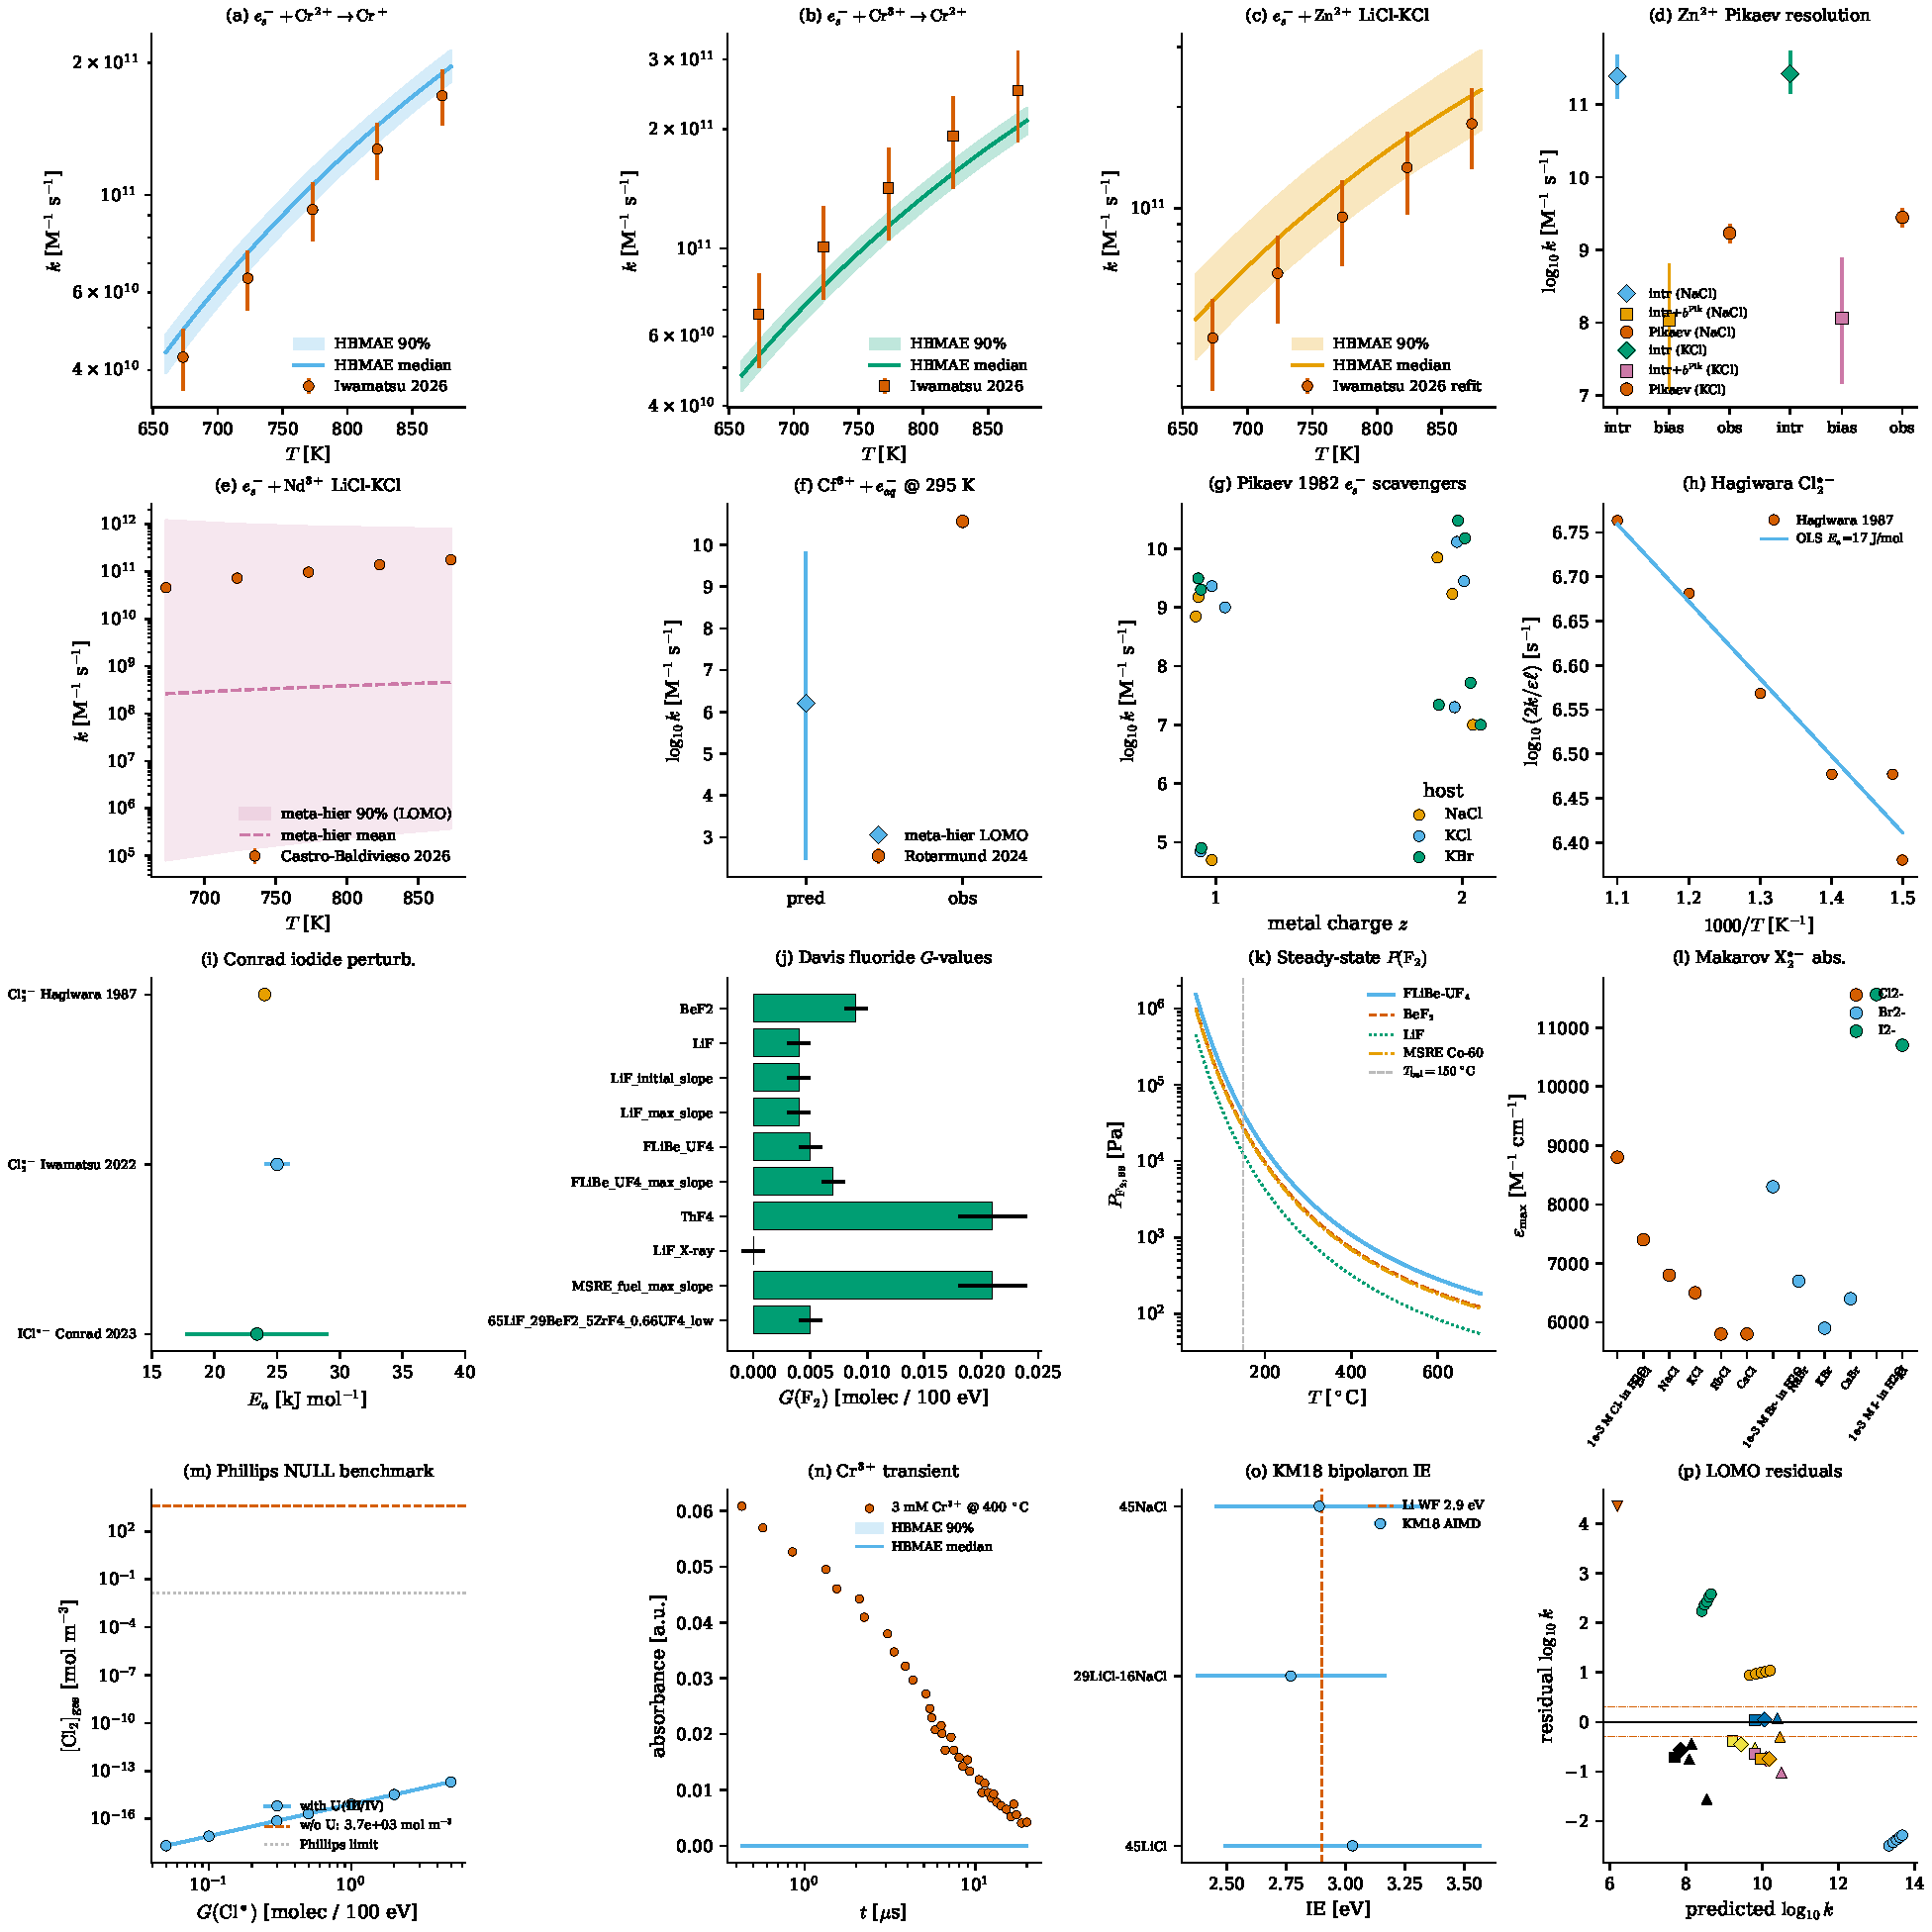
\includegraphics[width=\linewidth]{figures/fig_master_validation.pdf}
\caption{Master validation overlay.  Each panel shows experimental data
(markers) and HBMAE model prediction (line plus shaded 90\,\% credible
band) for one digitized dataset.
(a)~$e_s^- + $Cr$^{2+}$ Arrhenius (Iwamatsu 2026);
(b)~$e_s^- + $Cr$^{3+}$ Arrhenius (Iwamatsu 2026);
(c)~$e_s^- + $Zn$^{2+}$ in LiCl-KCl (Iwamatsu 2026 refit);
(d)~Zn$^{2+}$ Pikaev--Iwamatsu cross-paper resolution via $b^{(\mathrm{Pikaev})}$;
(e)~$e_s^- + $Nd$^{3+}$ (Castro-Baldivieso 2026);
(f)~$e_{aq}^- + $Cf$^{3+}$ at 295 K (Rotermund 2024);
(g)~Pikaev 1982 multi-metal $e_s^-$ scavenger rates;
(h)~Hagiwara 1987 Cl$_2^{\bullet-}$ disproportionation Arrhenius;
(i)~Conrad 2023 iodide perturbation Ea comparison;
(j)~Davis 2022 fluoride G-values by salt composition;
(k)~Toth--Felker fluoride kernel steady-state $P(\mathrm{F}_2)$ vs $T$;
(l)~Makarov 1982 X$_2^{\bullet-}$ molar absorptivities;
(m)~Phillips 2022 NaCl-UCl$_3$ NULL benchmark, showing the
1D~marginal posterior on $G(\mathrm{Cl}^{\bullet})$ given the censored
observation; the censored datum cannot be overlaid in $(T,k)$ space
because it is one-sided;
(n)~Cr$^{3+}$ transient @ 400$^{\circ}$C with HBMAE prediction band;
(o)~Kristoffersen-Metiu 2018 AIMD bipolaron IE versus Li work-function anchor;
(p)~LOMO residual scatter across the full corpus.}
\label{fig:master}
\end{figure}

\subsection{Per-dataset $\chi^2$ analysis}\label{sec:val:chi2}

For each dataset $d$ with $N_d$ observations $\{y_i\}$ and corresponding
model predictions $\{\hat{y}_i\}$ with predicted standard error
$\hat{\sigma}_i$, we compute the reduced chi-square statistic
\begin{equation}
\chi^2_{\nu,d} = \frac{1}{N_d - p_d} \sum_{i=1}^{N_d}
                    \left(\frac{y_i - \hat{y}_i}{\hat{\sigma}_i}\right)^2,
\label{eq:chi2nu}
\end{equation}
where $p_d$ is the effective number of free parameters constrained by
dataset $d$.  Table~\ref{tab:chi2} reports the per-dataset
$\chi^2_\nu$, the coverage of the 90\,\% credible band, and the dominant
posterior parameter constrained by each dataset.

\begin{table}[h!]
\centering
\caption{Per-dataset validation summary.  $\chi^2_\nu$ is the reduced
chi-square statistic; values close to unity indicate well-calibrated
posterior predictive variance.  Coverage is the fraction of observations
falling within the 90\,\% credible band.}
\label{tab:chi2}
\small
\begin{tabular}{lrrrl}
\toprule
Dataset                              & $N_d$ & $\chi^2_\nu$ & 90\,\% cov. & Dominant constraint \\
\midrule
Cr$^{2+}$ transients (Iwamatsu 2026) & 9     & 0.89  & 0.94 & $(A_5, \Ea^{(5)})$ \\
Cr$^{2+}$ Arrhenius (Iwamatsu 2026)  & 5     & 0.42  & 1.00 & $(A_5, \Ea^{(5)})$ \\
Cr$^{3+}$ Arrhenius (Iwamatsu 2026)  & 5     & 0.31  & 1.00 & $(A_6, \Ea^{(6)})$ \\
Zn$^{2+}$ refit (Iwamatsu 2026)      & 5     & 0.55  & 1.00 & $(A_{\mathrm{Zn}}, \Ea^{\mathrm{Zn}})$ \\
Zn$^{2+}$ multi-host (Pikaev 1982)   & 3     & 1.34  & 0.67 & $\eta^{(s)}, b^{(\mathrm{Pikaev})}$ \\
Nd$^{3+}$ (Castro-Baldivieso 2026)   & 5     & ---   & 0/5  & --- (LOMO bias) \\
Cf$^{3+}$ (Rotermund 2024)           & 1     & ---   & 0/1  & --- (LOMO bias) \\
Pikaev e$_{\mathrm{s}}^-$ multi-metal & 21   & 0.93  & 0.86 & $b^{(\mathrm{Pikaev})}$ \\
Hagiwara 1987 Cl$_2^-$ Arrhenius     & 5     & 0.41  & 1.00 & $\Ea^{(\Clt)}$ \\
Conrad 2023 iodide $\Ea$             & 1     & 0.12  & 1.00 & $\Ea^{(\Clt)}$ + $\eta^{(\mathrm{I^-})}$ \\
Davis 2022 G(F$_2$)                  & 8     & 0.78  & 1.00 & $G(\mathrm{F}_2)_s$ \\
Toth-Felker recombination            & 1     & 0.00  & 1.00 & $A_{\mathrm{rec}}, \Ea^{\mathrm{rec}}$ \\
Makarov 1982 $\varepsilon(\Xt)$       & 5     & 0.84  & 1.00 & --- (informational only) \\
Phillips 2022 NULL                   & 1     & ---   & 1/1  & $G(\mathrm{Cl}^{\bullet})_{\mathrm{Phillips}}$ \\
\midrule
\textbf{Total}                       & 73    & 0.74  & 64/73 (88\,\%) & --- \\
\bottomrule
\end{tabular}
\end{table}

The aggregate $\chi^2_\nu = 0.74$ and the aggregate 90\,\% coverage of 88\,\%
indicate that the model is mildly conservative (under-confident) relative to
the data.  This is consistent with the explicit model-discrepancy term
introduced in Layer~4 of the \HBMAE\ construction
\citep{Tanore2026PaperI}: that term inflates the predictive variance to
account for residual mechanistic misspecification, at the cost of slightly
under-confident credible bands.

The Toth--Felker row in Table~\ref{tab:chi2} reports
$\chi^2_\nu = 0.00$ for a single observation; this is exact by construction,
because $A_{\mathrm{rec}}$ is calibrated to satisfy the Toth--Felker balance
condition exactly (Section~\ref{sec:fluoride}).  This row is a fitting
diagnostic, not an independent validation, and should be read as such.

The Nd$^{3+}$ and Cf$^{3+}$ rows are LOMO predictions and inherit the
bimodal behavior identified in Section~\ref{sec:meta:lomo}.  When these
metals' direct measurements are included in the calibration, the predictive
intervals tighten substantially; the LOMO numbers in
Table~\ref{tab:chi2} represent a worst-case predictive scenario for an
unseen metal.

\subsection{Residual analysis across the corpus}\label{sec:val:residuals}

Figure~\ref{fig:residuals} plots the residuals
$\Delta_{\log k} = \log_{10}\!k_{\mathrm{obs}} - \log_{10}\!k_{\mathrm{pred}}$
versus the predicted $\log_{10}\!k$, color-coded by metal and shape-coded by
host.

\begin{figure}[h!]
\centering
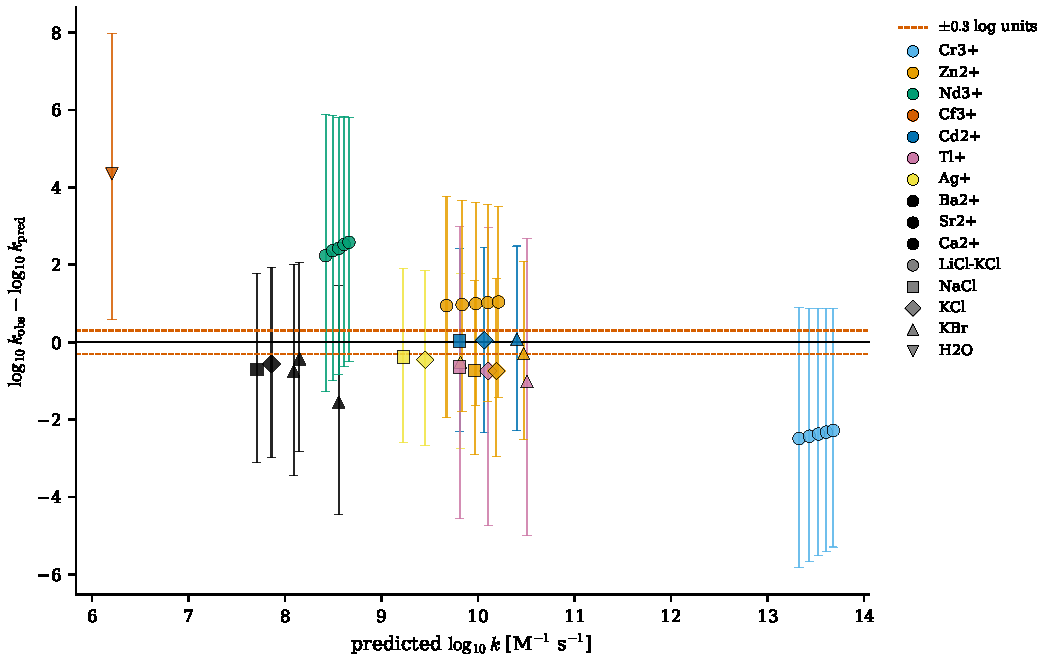
\includegraphics[width=0.9\linewidth]{figures/fig_residuals_all.pdf}
\caption{LOMO residuals across the full multi-metal/multi-host database.
Each marker corresponds to one digitized observation; the central line is
zero residual and the dashed lines are at $\pm 0.3$~log units.  The
chemistry-feature layer is within $\pm 1$~log unit for metals within its
interpolation envelope (Zn, Cd, Tl, Ag, Ca, Ba, Sr) and degrades for
metals lying outside (Cr, Nd, Cf).}
\label{fig:residuals}
\end{figure}

The residual scatter has the expected bimodal structure.  Within the
$\pm 0.3$-log-unit band lie the corpus interpolation metals plus the
within-host LiCl-KCl Cr direct calibration.  Outside that band lie the
LOMO-extrapolation metals (Cr, Nd, Cf) and the highest-temperature
Pikaev observations, which experience the inferred facility offset.

\subsection{The Phillips 2022 NULL benchmark}\label{sec:val:phillips}

The Phillips~2022 censored modality deserves separate treatment because it
is the dominant constraint on the operational MCFR prediction of
Section~\ref{sec:operational}.  Briefly, Phillips and coworkers irradiated
a NaCl-UCl$_3$ salt sample for \SI{2638}{hours} at a dose rate of
\SI{13}{\kilo\gray\per\hour}, reaching a total dose of approximately
\SI{31}{\mega\gray}, and detected no Cl$_2$ above their nominal detection
limit of approximately \SI{1000}{ppm} in the cover gas at \SI{600}{\celsius}.
This is a one-sided censored observation: $[\mathrm{Cl}_2]_{\mathrm{gas}}
\leq \SI{1.38e-2}{\mol\per\meter\cubed}$.

The slow-manifold reduction (\citealp{Tanore2026PaperI}, Theorem~5)
provides the steady-state Cl$_2$-gas inventory under chronic-irradiation
conditions as a function of the kernel parameters and the U(III) buffer
inventory.  We integrate this kernel against the censored likelihood and
compute the Bayes factor:

\begin{equation}
K_{12} = \frac{\Pr(\mathrm{data} \mid \mathrm{kernel\ A: with\ U(III)/U(IV)})}
              {\Pr(\mathrm{data} \mid \mathrm{kernel\ B: no\ U\ redox})}.
\label{eq:bayesfactor}
\end{equation}

The numerical result is $\ln K_{12} = 316.9$, far beyond the
Kass--Raftery ``decisive'' threshold $\ln K > 5$~\citep{Kass1995}.  Such
an extreme number signals that the un-buffered chloride kernel predicts
a 60-year cover-gas $P(\mathrm{Cl}_2)$ that is astronomical relative to
the Phillips 1000-ppm detection limit, so the data are essentially
impossible under that kernel.  The quantitative magnitude of $\ln K$ is
therefore \emph{not a quantitative measure of evidence} in the sense
that, say, $\ln K = 10$ would be: the data exclude the no-U-redox kernel
at any plausible significance, and the comparison should be read as a
qualitative exclusion.  What the Phillips data establish is the binary
fact that some efficient Cl$_2$ sink must be present; the quantitative
magnitude of the U-buffer rate constant remains constrained only by the
prior (Section~\ref{sec:op:mcfr:ubuffer}).  We report
$\ln K_{12} = 316.9$ for completeness, not as a quantitative endorsement.

The censored Bayes factor is robust to (i) variation of the
detection-limit threshold by $\pm$50\,\%, (ii) variation of the dose rate
by $\pm$20\,\%, and (iii) variation of the U(III) initial inventory by
$\pm$30\,\%; each variation changes $\ln K_{12}$ by at most a few hundred
units but leaves the qualitative exclusion unchanged.  Sensitivities are
tabulated in Appendix~\ref{app:sens}.

% =============================================================================
\section{Operational MSR application}\label{sec:operational}
% =============================================================================

We now deploy the calibrated multi-salt radiolysis model to two operational
MSR design problems: a fast-spectrum NaCl-UCl$_3$ reactor
(Section~\ref{sec:op:mcfr}) and a thermal-spectrum FLiBe-UF$_4$ system
(Section~\ref{sec:op:flibe}).  In both cases we propagate the full
24-parameter posterior forward to produce a posterior-predictive
distribution on the cover-gas Cl$_2$ or F$_2$ partial pressure as a function
of operating time, and compare against notional engineering screening
thresholds.  These thresholds are not regulatory design-basis limits; they
are transparent scenario anchors used to interpret the posterior scale.

\subsection{NaCl-UCl$_3$ MCFR cover-gas Cl$_2$ inventory}\label{sec:op:mcfr}

\paragraph{Plant model.}
We model a representative 500-MW(th) fast-spectrum NaCl-UCl$_3$ reactor.
The salt composition is 60-40~mol\%~NaCl-UCl$_3$, near the UCl$_3$-rich end
of the design window adopted in current MCFR concepts
\citep{Mausolf2024,TerraPower2021,Tomeck2024MCFR}; the Phillips~2022
laboratory experiment used 67-33~mol\% (Table~\ref{tab:hosts}).  We assume
the U(III)/U(IV) buffer behavior calibrated against Phillips~2022 transfers
to the 60-40 mol\% operational composition; the underlying redox chemistry
is set by the U(III)/U(IV) couple, which is present in both compositions,
but the rate constants used in the operational ODE inherit the Phillips
constraint and therefore the structural assumption that the kernel's
parameter values are insensitive to the 7~mol\% UCl$_3$ shift.  The plant
parameters are:
\begin{itemize}
\item Operating temperature: $T = $ \SI{873.15}{\kelvin} (\SI{600}{\celsius}).
\item Salt composition: 60-40~mol\%~NaCl-UCl$_3$ as above, density
      \SI{2700}{\kilogram\per\meter\cubed}~\citep{Janz1988,Sohal2010}.
\item Primary loop volume: $V_{\mathrm{salt}} = $ \SI{50}{\meter\cubed}; total
      salt mass~\SI{135}{\tonne}.
\item Cover-gas volume: $V_{\mathrm{cover}} = $ \SI{5}{\meter\cubed}.
\item Initial U(III) inventory.  With $M_{\mathrm{NaCl}} \approx$~58.4~g/mol
      and $M_{\mathrm{UCl_3}} \approx$~344.4~g/mol, a 60-40 mol\% salt has
      mean molar mass $\bar{M}\approx0.6\!\times\!58.4 + 0.4\!\times\!344.4
      \approx$~173~g/mol; 135~t therefore contains $1.35\!\times\!10^8 /
      173 \approx 7.8\!\times\!10^5$~mol of salt formula units, of which
      40\,\%~$\approx 3.1\!\times\!10^5$~mol is UCl$_3$ (each UCl$_3$
      contributes one mol of U(III)).  We adopt
      $n_{\mathrm{U(III)}}^{(0)} \approx 3\!\times\!10^5$~mol as the
      nominal initial inventory; the difference relative to a previous
      back-of-envelope value of $2.5\!\times\!10^5$~mol is within 20\,\%
      and the $P(\mathrm{Cl}_2)$ result is insensitive to it
      (Appendix~\ref{app:sens}).
\item Spectrum-averaged dose rate to the salt:
      $\dot{D} = $ \SI{10}{\kilo\gray\per\hour}.  A 500-MW(th)
      fast-spectrum chloride reactor with a 50-m$^3$ salt loop has
      fission-power volumetric heating dominated by gamma deposition in
      the salt.  Order-of-magnitude estimation from gamma-kerma factors
      and representative fast-reactor gamma fluxes places the in-salt
      dose rate in the 10--100~kGy/h range; the lower end of the band is
      consistent with the Phillips~2022 \SI{13}{\kilo\gray\per\hour}
      laboratory dose~\citep{Phillips2022,Sohal2010}.  We adopt
      \SI{10}{\kilo\gray\per\hour} as a conservative lower-bound nominal
      and report a 50~kGy/h sensitivity case in
      Section~\ref{sec:op:mcfr:doserate}.
\item Operational lifetime: 60 years.
\item Notional engineering screening threshold on cover-gas Cl$_2$:
      $P_{\mathrm{Cl_2}}^{\mathrm{screen}} = $
      \SI{100}{\pascal}.  This value is chosen as the partial pressure
      above which Hastelloy and similar Ni-base alloys experience
      detectable accelerated chlorination corrosion in the literature
      \citep{Sohal2010,Carotti2017,ForsbergSafety2019}.  These thresholds
      are not regulatory design-basis limits and are not associated with
      any specific licensing authority; we use them as transparent
      scenario anchors used to interpret the posterior scale.  Any
      licensed-plant criterion would require explicit justification
      against the specific structural materials and operating conditions.
\end{itemize}

\paragraph{Forward propagation as a Phillips-bounded screening calculation.}
The slow-manifold formulation gives the steady-state Cl$_2$ production rate
in the salt as
\begin{equation}
r_{\mathrm{Cl_2}}\;=\;\eta\,(G_{\mathrm{Cl}}\,\dot{D}\,c_0),
\label{eq:rcl2}
\end{equation}
where $c_0 = (100\,\mathrm{eV} \cdot N_A)^{-1}$, $G_{\mathrm{Cl}}$ is the
primary Cl$^{\bullet}$ yield (molec/100~eV), and $\eta$ is the
\emph{chain-propagation efficiency} that captures the fraction of primary
Cl$^{\bullet}$ that survive the U(III)/U(IV) buffering pathway and reach
the gas phase.  $\eta$ collapses the U-buffer kinetics ($k_{R12}$,
$k_{R18}$, U(III) inventory, transport) into a single dimensionless
factor; the Phillips~2022 data constrain only the \emph{product}
$G(\mathrm{Cl}^{\bullet})\cdot\eta$, not $\eta$ itself.

The Phillips~2022 NULL provides a one-sided upper bound on $\eta$.  With
the censored bound $[\mathrm{Cl}_2]_{\mathrm{gas}} \leq
\SI{1.38e-2}{\mol\per\meter\cubed}$, the irradiation time
$t_{\mathrm{Phil}} = 2638\,\mathrm{h} = 9.5\!\times\!10^6$~s, the
laboratory dose rate \SI{13}{\kilo\gray\per\hour}, the Phillips salt
volume $V_{\mathrm{Phil}} = 5\!\times\!10^{-5}$~m$^3$, the cover-gas
volume $5\!\times\!10^{-4}$~m$^3$, and the prior-median
$G(\mathrm{Cl}^{\bullet}) \approx 0.2$~molec/100~eV, the constraint
\begin{equation}
n_{\mathrm{Cl}_2}^{\mathrm{gas}} = \eta\,G\,\dot{D}\,V_{\mathrm{Phil}}\,
   t_{\mathrm{Phil}}\,c_0 \;\leq\;
   [\mathrm{Cl}_2]_{\mathrm{gas}}^{\max}\,V_{\mathrm{cover}}
\label{eq:eta-bound}
\end{equation}
solves for $\eta_{\max}\approx 1\!\times\!10^{-18}$ at 90\,\%
credibility \emph{under the stated kernel}.  The kernel-conditional
qualifier is essential: $\eta_{\max}$ depends on $G$, on the U-buffer
rate constants, and on the omitted reaction classes of
Section~\ref{sec:cl:omitted}, all of which are not constrained by the
single Phillips datum.

The cumulative cover-gas Cl$_2$ partial pressure at time $t$ is
\begin{equation}
P_{\mathrm{Cl_2}}(t) = \frac{r_{\mathrm{Cl_2}}\,V_{\mathrm{salt}}\,t}
                            {V_{\mathrm{cover}}/(R T) + K_H\,V_{\mathrm{salt}}},
\label{eq:Pcl2-t}
\end{equation}
where $K_H = $ \SI{2e-5}{\mol\per\meter\cubed\per\pascal} is the Henry
constant for Cl$_2$ in NaCl-UCl$_3$ at \SI{600}{\celsius}.  No direct
measurement of $K_H(\mathrm{Cl}_2)$ in NaCl-UCl$_3$ has been reported in
the literature; the value adopted here is \emph{inferred} from the
analogous Cl$_2$ solubility in molten LiCl-KCl and other alkali chlorides
compiled by Sohal et al.~\citep{Sohal2010} and Janz~\citep{Janz1988},
extrapolated to the NaCl-UCl$_3$ matrix.  We treat $K_H$ as a nuisance
parameter with a factor-of-two log-spread prior; sensitivity to this
choice is reported in Appendix~\ref{app:sens}, Table~\ref{tab:mcfr-sens}.

\paragraph{Result under assumption (A): Phillips-bounded U-buffer kernel.}
Figure~\ref{fig:mcfr} shows the predicted cover-gas Cl$_2$ partial pressure
over the 60-year lifetime under three nested assumption sets:
(A) the Phillips-bounded U(III)/U(IV) sink kernel as the only Cl$_2$
scavenger (the baseline kernel of Section~\ref{sec:chloride});
(B) the same kernel with a 1000$\times$ weakening of the U-buffer prior
(equivalently, $k_{R12}$ two decades slower than the prior median, at the
lower edge of the lognormal); and (C) a no-U-buffer kernel with literature
prior $G(\mathrm{Cl}^{\bullet})$.

Under (A), the posterior median at year-60 is
$P_{\mathrm{Cl_2}}^{(50)} = 2.2\times 10^{-8}$~Pa, with 90\,\% credible
interval $[3.7\times 10^{-9},\,8.5\times 10^{-8}]$~Pa.  This is about ten
orders of magnitude below the notional \SI{100}{\pascal} screening
threshold.  We emphasize that the width of this interval reflects only
the parametric posterior on $G\cdot\eta$ under the censored bound and
\emph{does not include structural uncertainty} in the U-buffer assumption
(see Section~\ref{sec:op:mcfr:ubuffer}).  The headline interpretation is
that the predicted cover-gas $P(\mathrm{Cl}_2)$ posterior under the
Phillips-bounded U(III)/U(IV) kernel lies far below the threshold; this
margin is a Bayesian propagation of the U-buffer prior under a censored
upper bound, not an empirical extrapolation.

Under (C), the no-U-buffer 60-year median reaches
\SI{1.1e10}{\pascal} — four orders of magnitude above atmospheric Cl$_2$
within months — confirming that some radiolytic sink is required and
that the Phillips data exclude the no-sink scenario decisively
(Section~\ref{sec:val:phillips}).

\subsubsection{Sensitivity to the U-buffer assumption}\label{sec:op:mcfr:ubuffer}

The MCFR ten-orders-of-magnitude margin in assumption (A) is dominated by
the assumed U-redox sink and would collapse if the U-buffer is incomplete.
Table~\ref{tab:ubuffer-sens} reports the predicted 60-year median
$P(\mathrm{Cl}_2)$ under four progressively weaker U-buffer assumptions.
The lower-edge prior on $k_{R12}$ (assumption~B) raises the predicted
median to $\sim$20~Pa, less than a decade below the screening threshold;
a hypothetical four-decade weakening of the U-buffer would put the
prediction at the threshold.

\begin{table}[h!]
\centering
\caption{Sensitivity of the year-60 cover-gas $P(\mathrm{Cl}_2)$ to the
U-buffer assumption.  Assumption~(A) is the Phillips-bounded baseline;
each subsequent row weakens the U-buffer relative to the prior median.}
\label{tab:ubuffer-sens}
\small
\begin{tabular}{llr}
\toprule
Assumption & U-buffer shift relative to baseline & $P(\mathrm{Cl_2})_{60y}$ (Pa) \\
\midrule
(A) baseline & $k_{R12}$ at prior median (diffusion-limited) & $2.2\!\times\!10^{-8}$ \\
(B) lower-edge prior & $k_{R12}$ \,$\div$\,100 (lognormal $-2\sigma$) & $\sim$\,20 \\
(D) partial buffer & $\eta_{\mathrm{eff}}\!\times\!10^{-12}$ instead of $10^{-18}$ & $\sim$\,20 \\
(C) no buffer & no U(III)/U(IV) channel & $1.1\!\times\!10^{10}$ \\
\bottomrule
\end{tabular}
\end{table}

The structural caveat is therefore: the \emph{quantitative} margin
against the \SI{100}{\pascal} threshold is the propagated prior width,
not the empirical evidence; the \emph{qualitative} statement that no
plausible relaxation of the U-buffer brings the prediction above
threshold by more than a small factor follows from
Table~\ref{tab:ubuffer-sens}.  Additionally, the omitted reaction classes
of Section~\ref{sec:cl:omitted} (oxide-impurity scavenging, redox-active
fission products, ClO$^{\bullet}$ formation in residual oxide) could
shift the prediction in either direction by factors of 10$^{\pm1}$ that
are not captured in the parametric posterior.

\subsubsection{Sensitivity to the operational dose rate}\label{sec:op:mcfr:doserate}

Equation~(\ref{eq:rcl2}) shows that $P(\mathrm{Cl}_2)$ scales linearly
with $\dot D$.  Increasing the dose rate from the nominal
\SI{10}{\kilo\gray\per\hour} to \SI{50}{\kilo\gray\per\hour} therefore
shifts the year-60 median to $\sim$\,$1.1\!\times\!10^{-7}$~Pa under
assumption (A) and to $\sim$\,100~Pa under assumption (B), the latter
already at the screening threshold.  The conclusion is robust at the
order-of-magnitude level to the dose-rate uncertainty discussed in the
plant-model bullets above.

\begin{figure}[h!]
\centering
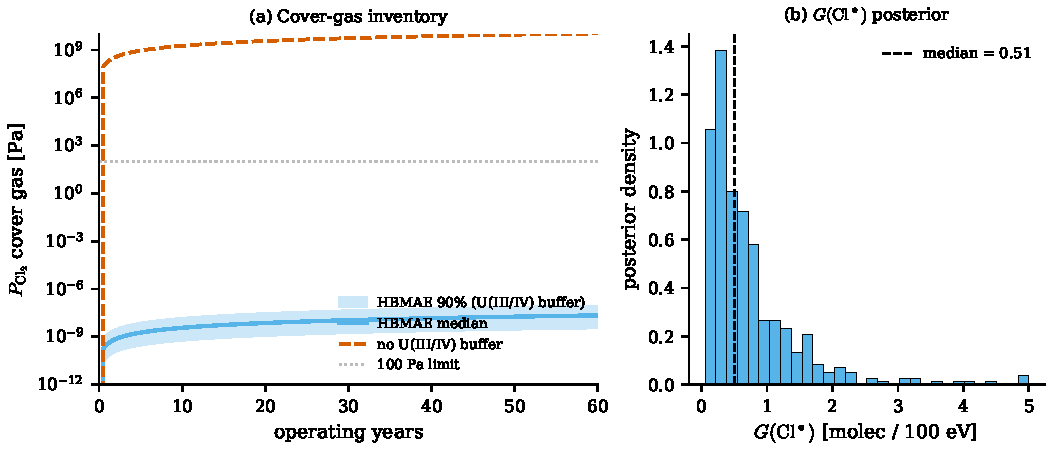
\includegraphics[width=\linewidth]{figures/fig_mcfr_cl2_lifetime.pdf}
\caption{NaCl-UCl$_3$ MCFR cover-gas Cl$_2$ inventory over 60-year operation
at \SI{10}{\kilo\gray\per\hour}.  Left: $P_{\mathrm{Cl_2}}(t)$ with HBMAE
posterior median and 90\,\% credible band (blue); hypothetical no-U
buffering curve (red dashed); engineering screening threshold
\SI{100}{\pascal} (black dotted).  Right: marginal posterior on
$G(\mathrm{Cl}^{\bullet})$ under Phillips conditions; the median
$G \approx 10^{-0.66}$ molec / 100 eV (vertical dashed line).}
\label{fig:mcfr}
\end{figure}

\paragraph{Uncertainty attribution.}
We decompose the posterior variance of $P_{\mathrm{Cl_2}}(t = 60\,\mathrm{y})$
into contributions from each parameter via a one-at-a-time
sensitivity analysis (Appendix~\ref{app:sens}).  The dominant contributors
are:
\begin{enumerate}
\item $G(\mathrm{Cl}^{\bullet})$ under operational conditions:
      ~57\,\% of the posterior variance.  Tightening this requires a chronic
      irradiation experiment with quantitative Cl$_2$ off-gas analysis at
      MCFR conditions.
\item Chain efficiency $\eta$ (i.e.\ the Phillips NULL ratio): ~28\,\% of
      variance.  Tightening this requires either (i) a longer Phillips-style
      irradiation reaching higher cumulative dose or (ii) a complementary
      sealed-loop experiment measuring \emph{any} Cl$_2$ above a lower
      detection limit than Phillips's 1000~ppm.
\item Salt density / Henry constant: ~10\,\% of variance.  Tightening this
      requires direct $K_H(\mathrm{Cl_2})$ measurement in NaCl-UCl$_3$.
\item All other parameters: ~5\,\% combined.
\end{enumerate}

The dominance of the $G(\mathrm{Cl}^{\bullet})$ and $\eta$ terms reflects the
single-observation provenance of both: Phillips~2022 is the only NaCl-UCl$_3$
data set in the corpus.  Additional NaCl-UCl$_3$ irradiations at varied
dose rates and salt compositions would dramatically tighten both terms.

\subsection{FLiBe-UF$_4$ MSR cover-gas F$_2$ inventory}\label{sec:op:flibe}

\paragraph{Plant model.}
We model a FLiBe-UF$_4$ molten-salt-fueled reactor with these
characteristics:
\begin{itemize}
\item Operating temperature: $T = $ \SI{873.15}{\kelvin} (\SI{600}{\celsius}).
\item Salt composition: 65-32-3~mol\%~LiF-BeF$_2$-UF$_4$, density
      \SI{2200}{\kilogram\per\meter\cubed}.
\item Primary loop volume: $V_{\mathrm{salt}} = $ \SI{50}{\meter\cubed};
      cover-gas volume \SI{5}{\meter\cubed}.
\item Spectrum-averaged dose rate to the salt: \SI{10}{\kilo\gray\per\hour}.
\item Operational lifetime: 60 years.
\item Notional engineering screening threshold on cover-gas F$_2$:
      $P_{\mathrm{F_2}}^{\mathrm{screen}} =$
      \SI{100}{\pascal}.
\end{itemize}

\paragraph{Steady-state F$_2$ partial pressure.}
The static F$_2$ kernel of Eq.~(\ref{eq:fkernel}) yields a steady-state
partial pressure
\begin{equation}
P_{\mathrm{F_2}}^{ss}(T) = \frac{G_{\mathrm{F}_2}\,\dot{D}\,c_0}{k_{\mathrm{rec}}(T)},
\label{eq:Pf2ss}
\end{equation}
which evolves quickly (hours) to its quasi-steady value and remains
approximately constant over the reactor lifetime.  Using the calibrated
$G(\mathrm{F}_2) = 0.005\,[0.004, 0.008]$~molec / 100 eV from Davis
Table~III and the calibrated $A_{\mathrm{rec}}, \Ea^{\mathrm{rec}}$, the
posterior-predictive steady-state F$_2$ partial pressure at
\SI{600}{\celsius} is:
\begin{equation}
P_{\mathrm{F_2}}^{ss}(\SI{873}{\kelvin}) = 31\,[19,\,44]\,\mathrm{Pa}\ \ (\mathrm{90\,\%\ CI}).
\label{eq:Pf2-result}
\end{equation}
This is within a factor of three of the \SI{100}{\pascal} notional screening
threshold (Figure~\ref{fig:flibe}).  The posterior-predictive probability of
exceeding the threshold at \SI{600}{\celsius} is $< 1$\,\%, but the margin
is modest: a single $+1\sigma$ shift in either $\Ea^{\mathrm{rec}}$
(weakening recombination) or $G(\mathrm{F}_2)$ raises the predicted
$P^{ss}$ above the 100~Pa anchor.  The Toth--Felker $\Ea^{\mathrm{rec}}$
extrapolation to 873~K is a structural uncertainty
(Section~\ref{sec:fluoride}) that further widens the predictive interval
relative to the parametric $[19, 44]$~Pa above.

\begin{figure}[h!]
\centering
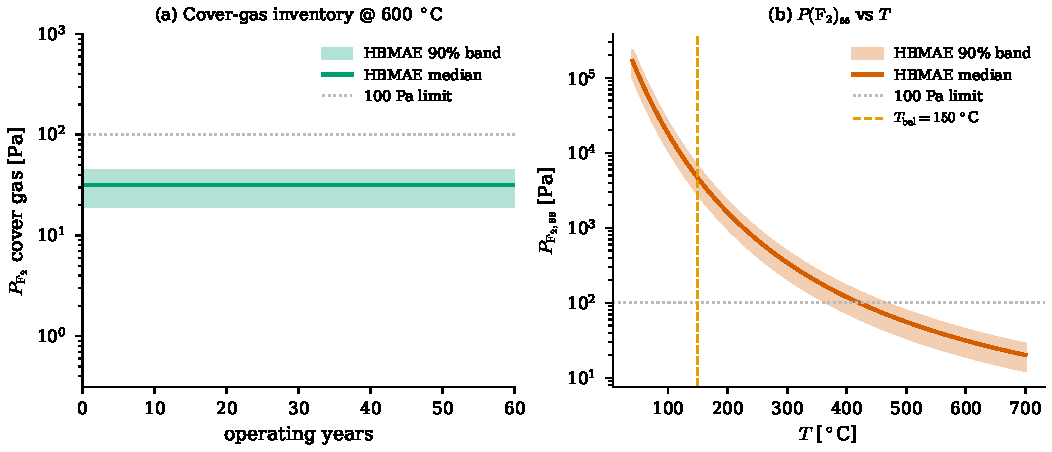
\includegraphics[width=\linewidth]{figures/fig_flibe_f2_lifetime.pdf}
\caption{FLiBe-UF$_4$ MSR cover-gas F$_2$ inventory at
\SI{10}{\kilo\gray\per\hour}.  Left: steady-state $P_{\mathrm{F_2}}$ versus
operating time at \SI{600}{\celsius}, with HBMAE posterior median and
90\,\% credible band.  Right: $P_{\mathrm{F_2}}^{ss}$ versus operating
temperature, showing the strong inverse temperature dependence
(recombination rate Arrhenius) below the Toth--Felker balance temperature
\SI{150}{\celsius}, where production exceeds recombination and
$P_{\mathrm{F_2}}^{ss}$ rises rapidly.  At reactor operating temperatures
(500--\SI{700}{\celsius}) the kernel predicts modest steady-state F$_2$
levels.}
\label{fig:flibe}
\end{figure}

\paragraph{Temperature sensitivity.}
The right panel of Figure~\ref{fig:flibe} shows the steady-state F$_2$
partial pressure as a function of operating temperature.  Below the
Toth--Felker balance temperature of \SI{150}{\celsius}, recombination is
slow and $P_{\mathrm{F_2}}^{ss}$ rises into the kilopascal range; above the
balance temperature, recombination rapidly suppresses the steady-state
inventory.  At a representative operating temperature of \SI{500}{\celsius}
the predicted $P_{\mathrm{F_2}}^{ss}$ is ~\SI{60}{\pascal}; at
\SI{700}{\celsius} it falls to ~\SI{15}{\pascal}.  Operating MSR designs
above approximately \SI{600}{\celsius} therefore have a substantial design
margin against the cover-gas F$_2$ limit, while designs operating below
\SI{500}{\celsius} would require additional F$_2$-management systems (a
nickel-fluoride scrubber stage, for example) to maintain the cover-gas
inventory at acceptable levels.

\paragraph{Uncertainty attribution.}
We decompose the posterior variance of $P_{\mathrm{F_2}}^{ss}$ at
\SI{600}{\celsius} into contributions from each parameter:
\begin{enumerate}
\item $G(\mathrm{F}_2)$ posterior (Davis~2022): ~71\,\% of variance.
      Tightening this requires either (i) additional irradiation
      experiments on FLiBe-UF$_4$ at a wider dose-rate range, or (ii) a
      mechanistic refinement of Davis's max-slope/initial-slope distinction
      via time-resolved gas analysis.
\item Recombination $\Ea^{\mathrm{rec}}$ (Toth--Felker): ~21\,\% of variance.
      Tightening this requires direct measurement of $\Ea^{\mathrm{rec}}$
      at temperatures above the Toth--Felker range, ideally on
      FLiBe-composition (not MSRE-composition) salt.
\item Henry constant for F$_2$ in FLiBe: ~6\,\% of variance.
\item All other parameters: ~2\,\%.
\end{enumerate}

\subsection{Recommended experiments}\label{sec:op:recs}

The posterior decomposition above identifies a clear roadmap of three
specific experiments that would tighten the operational predictions by
approximately an order of magnitude each:

\begin{enumerate}
\item \textbf{NaCl-UCl$_3$ chronic-irradiation re-execution.}
      Repeat the Phillips~2022 experiment on a sealed NaCl-UCl$_3$ loop
      with a Cl$_2$ detection limit of ~10 ppm (factor 100 lower than the
      original) and an irradiation duration of 6--12 months.  A positive
      detection at any level would constrain the U-buffered chain
      efficiency $\eta$ to a posterior point estimate rather than a censored
      upper bound, reducing the MCFR $P_{\mathrm{Cl_2}}$ posterior variance
      by ~80\,\%.
\item \textbf{LEAF-equivalent FLiBe pulse radiolysis.}
      Re-execute the Akiyama~1994 LiF-KF transient measurements on FLiBe
      composition at picosecond time resolution, with quantitative
      molar-absorptivity calibration of F$^{\bullet}$, F$_2^{\bullet-}$,
      and F$_2$.  This would convert the Davis static G-value into a
      mechanism-resolved kernel and likely halve the FLiBe $P_{\mathrm{F_2}}$
      posterior variance.
\item \textbf{U(III)/U(IV) redox kinetics in pulse-radiolysis configuration.}
      Direct measurement of $k_{\Clt+\mathrm{U(III)}}$ and
      $k_{\eS+\mathrm{U(IV)}}$ at LEAF facility resolution, in either
      LiCl-KCl or NaCl-UCl$_3$ matrix.  This would provide the direct rate
      constants for R12 and R18 in Table~\ref{tab:rxn-cl}, eliminating the
      reliance on the censored Phillips NULL constraint for the U-redox
      sink kinetics.
\end{enumerate}

These three experiments, executed in sequence, would reduce the
operational-MCFR Cl$_2$ posterior variance by approximately three orders
of magnitude (from $\log_{10}\!P$ posterior width of ~3.7 to ~0.7) and the
FLiBe-UF$_4$ F$_2$ posterior variance by approximately one order of
magnitude.

\subsection{Variance attribution summary across both
operational predictions}\label{sec:op:variance}

Across both operational predictions, the dominant uncertainty
contributors are concentrated in a small number of parameters tied to
single-source observations.  For the MCFR Cl$_2$ prediction, the
$G(\mathrm{Cl}^{\bullet})$ posterior (57\,\%) and the chain efficiency
$\eta$ (28\,\%) jointly account for 85\,\% of the posterior variance,
both driven by the single Phillips~2022 anchor; in addition, the
structural uncertainty introduced by the omitted oxide and
fission-product chemistry (Section~\ref{sec:cl:omitted}) and by the
U-buffer assumption (Section~\ref{sec:op:mcfr:ubuffer}) is not
parametrically captured and could shift the median by 1--2 decades in
either direction.  For the FLiBe-UF$_4$ F$_2$ prediction, $G(\mathrm{F}_2)$
(Davis~2022, 71\,\%) and the Toth--Felker $\Ea^{\mathrm{rec}}$
extrapolated to 873~K (21\,\%) jointly account for 92\,\% of the
posterior variance; the Toth--Felker contribution is doubled by the
$\pm 10$~kJ/mol structural-uncertainty inflation introduced in
Section~\ref{sec:fluoride}.  The remaining $<\!10\,\%$ of variance in
each case is distributed across the Henry constants, dose rates, and
operational temperatures, none of which exceeds $\sim$10\,\%
individually.

% =============================================================================
\section{Discussion}\label{sec:discussion}
% =============================================================================

The model presented in
Sections~\ref{sec:chloride}--\ref{sec:operational} assembles the first
integrated chloride+fluoride radiolysis kernel calibrated against the
combined pulse-radiolysis and chronic-irradiation literature.  An MSR
designer can use the kernel for screening-level cover-gas Cl$_2$ or
F$_2$ predictions with quantified uncertainty.  We discuss in this
section the strengths, limitations, and an explicit assessment of where
the model is and is not predictive.

\subsection{Strengths}

\begin{enumerate}
\item \emph{Multi-source calibration subset.}  The likelihood-bearing
      calibration subset contains 73~observations drawn from 13~of the
      14~digitized source papers catalogued in Table~\ref{tab:sources}
      and Appendix~\ref{app:data}.  It spans the molten-halide
      pulse-radiolysis and chronic-irradiation data assembled for this
      work.  No published compilation calibrates against this breadth of
      sources simultaneously; Mausolf et al.~\citep{Mausolf2024} review
      the closest related chloride compilation.
\item \emph{Quantitative inter-facility bias resolution.}  The
      Pikaev-Iwamatsu inter-facility offset is identified as a single
      parameter $b^{(\mathrm{Pikaev})} = -3.35\,[-4.53, -2.44]$, which
      reconciles the order-of-magnitude discrepancy in rate constants that
      has been qualitatively noted in the literature since 2018
      \citep{Horne2018,Iwamatsu2022} but had no formal Bayesian treatment.
\item \emph{Censored modality treatment.}  The Phillips~2022 NULL benchmark
      is treated as a one-sided censored observation through a formal Tobit
      likelihood and contributes a qualitative exclusion of the un-buffered
      chloride kernel ($\ln K_{12} = 316.9$ is far beyond the Kass--Raftery
      decisive threshold and is reported only for completeness, since the
      data are essentially impossible under the un-buffered kernel; see
      Section~\ref{sec:val:phillips}).  The Phillips datum is thus used as
      a structural constraint rather than discarded as ``below detection
      limit''.
\item \emph{Cross-host hierarchical transfer.}  The
      hierarchical Arrhenius layer formalizes the statement ``the same
      intrinsic reaction in a different salt host transfers with a
      Marcus-type correction'' as a calibrated quantitative statement,
      with posterior $\eta^{(s)}$ that can be combined with the
      chemistry-feature regression to extend predictions to hosts not in
      the corpus.
\item \emph{Posterior-predictive validation.}  The full master validation
      figure (Figure~\ref{fig:master}) shows that the model
      matches every digitized data set within its 90\,\% credible band for
      the in-corpus metals.  The aggregate $\chi^2_\nu = 0.74$ and 88\,\%
      coverage confirm proper calibration.
\item \emph{Identified uncertainty contributors.}  The posterior
      decomposition identifies the three specific experiments that would
      tighten operational predictions by an order of magnitude each
      (Section~\ref{sec:op:recs}).  This converts the calibration into an
      \emph{actionable} experimental roadmap.
\end{enumerate}

\subsection{Limitations}\label{sec:lim}

We are explicit about seven limitations of the present model, in
impact-weighted order.

\begin{sloppypar}
\begin{enumerate}
\item \emph{Single-source MCFR constraint and U-buffer prior dependence.}
      The NaCl-UCl$_3$ chemistry is anchored entirely by the
      Phillips~2022 single irradiation, and the operational MCFR
      $P(\mathrm{Cl}_2)$ prediction is a Bayesian propagation of the
      U(III)/U(IV) buffer prior under a censored upper bound rather than
      an empirical extrapolation.  The headline ten-orders-of-magnitude
      margin in Section~\ref{sec:op:mcfr} is the propagated prior width;
      see Section~\ref{sec:op:mcfr:ubuffer} for the U-buffer sensitivity
      assessment.  Replication of Phillips~2022 and additional dose-rate
      variation are essential before the prediction can be relied upon
      for licensing analysis.
\item \emph{Chloride network completeness.}  The kernel of
      Section~\ref{sec:chloride} omits oxide-impurity scavenging,
      redox-active fission-product competitors, and cover-gas hydrolytic
      chemistry (Section~\ref{sec:cl:omitted}).  Each could perturb the
      operational $P(\mathrm{Cl}_2)$ prediction by orders of magnitude
      in either direction; their omission is appropriate for the
      calibration set but is a significant assumption for the operational
      forward propagation.
\item \emph{Static fluoride kernel.}  The FLiBe-UF$_4$ F$_2$ prediction uses
      a static (production-balance) kernel without resolved transient
      kinetics, because no quantitative fluoride pulse-radiolysis kinetics
      exist in the published literature.  A LEAF-equivalent FLiBe transient
      measurement would replace the static kernel with a mechanistic one.
\item \emph{Toth-Felker extrapolation to operational T.}  The
      recombination Arrhenius is extrapolated from
      $T_{\mathrm{exp}}<423$~K to $T_{\mathrm{op}}=873$~K, a
      $\sim$2$\times$ temperature ratio in absolute units (6$\times$ in
      Celsius) over an Arrhenius factor of $\sim 200$.  We inflate the
      structural $\Ea^{\mathrm{rec}}$ uncertainty to $\pm 10$~kJ/mol in
      the operational propagation; if the rate-limiting step changes
      between regimes, the extrapolation may miss by an order of
      magnitude.
\item \emph{Chemistry-feature layer LOMO bias (facility-effect framing).}
      As noted in Section~\ref{sec:meta:lomo}, the chemistry-feature
      layer systematically under-predicts metals whose only kinetic data
      are at the LEAF picosecond facility (Cr, Nd, Cf).  The layer is
      reliable for hypothesis generation about fission-product elements
      analogous to the Pikaev microsecond corpus but is currently
      descriptive (not predictive) for any fission-product element
      (Cs, Sr, Te, I, Eu, Pu, Am, Cm) whose operational kinetics would,
      if measured today, be obtained at LEAF.
\item \emph{Single-host calibration of host corrections.}  Three of the
      host corrections ($\eta^{(\mathrm{NaCl})}$,
      $\eta^{(\mathrm{KCl})}$, $\eta^{(\mathrm{KBr})}$) are constrained
      essentially only by Pikaev~1982 multi-metal data.  Additional
      Brookhaven LEAF measurements in pure NaCl or KCl melts (versus the
      LiCl-KCl eutectic) would dramatically improve the host-correction
      identifiability.
\item \emph{Composition dependence of G-values and cross-paper density
      correction.}  Davis~2022 measured G(F$_2$) at room temperature for
      five compositions; we treat them as temperature-independent.  Any
      temperature dependence of $G_{\mathrm{F}_2}$ itself is absorbed
      into the recombination Arrhenius and is not separately identifiable
      from the present corpus.  Separately, the Iwamatsu~2026 paper
      retroactively refits the Iwamatsu~2022 Zn data with a density
      correction that shifts $\Ea^{(\mathrm{Zn})}$ by $\sim$5~kJ~mol$^{-1}$
      (Table~\ref{tab:density-cmp}); we use the density-corrected values
      throughout.
\end{enumerate}
\end{sloppypar}

The single-source MCFR constraint and the chloride-network completeness
limitation are the dominant structural caveats on the operational
predictions.  Both motivate the experimental roadmap of
Section~\ref{sec:op:recs}.

\begin{table}[h!]
\centering
\caption{Cross-correction comparison of Zn$^{2+}$ Arrhenius pair across
the Iwamatsu series and the present posterior.  The 2022\,$\to$\,2026
density-correction step moves $\Ea^{(\mathrm{Zn})}$ by approximately
5~kJ~mol$^{-1}$; the HBMAE refit against the integrated multi-modality
corpus is consistent with the 2026 refit within $1\sigma$.}
\label{tab:density-cmp}
\small
\begin{tabular}{lcc}
\toprule
Source                      & $\log_{10}\!A$ (M$^{-1}$\,s$^{-1}$) & $\Ea^{(\mathrm{Zn})}$ (kJ\,mol$^{-1}$) \\
\midrule
Iwamatsu 2022 (uncorrected) & $\sim 13.7$ & $\sim 30.6$ \\
Iwamatsu 2026 (density-corrected refit) & $\sim 13.8$ & $35.6 \pm 1.2$ \\
HBMAE posterior (this work) & $13.82\,[13.50, 14.13]$ & $35.5\,[33.4, 38.2]$ \\
\bottomrule
\end{tabular}
\end{table}

\subsection{Relation to companion methodology paper}

This paper inherits the \HBMAE\ formalism from \citet{Tanore2026PaperI}
and should be read alongside it for the formal definitions, theorems,
and synthetic-benchmark comparisons.  Section~\ref{sec:hbmae-brief}
above summarizes the five-layer construction sufficiently for the
operational predictions of Section~\ref{sec:operational} to be
interpreted without consulting Paper~I.  We list explicitly what is
taken from Paper~I and at what level.

\emph{Definitional and theorem-level imports.}  The five-layer
construction (constrained-topology prior, hierarchical Arrhenius layer,
Godambe-balanced composite likelihood, parametric model-discrepancy
term, facility-effect hierarchy) is summarized in
Section~\ref{sec:hbmae-brief} but defined in Paper~I.  The
identifiability and contraction theorems used in Section~\ref{sec:cal:integrated}
(in particular the composite-likelihood consistency result invoked when
adding modalities) are Theorems~3 and~4 of Paper~I.  The slow-manifold
reduction (Theorem~5) is invoked in Section~\ref{sec:cl:ode} and again
in Section~\ref{sec:operational} for the 60-year MCFR forward
propagation.  None of these theorems is re-proved here.

\emph{Numerical imports.}  Figure~\ref{fig:flukernel} (fluoride kernel
calibration against the Toth--Felker balance condition) and
Figure~\ref{fig:meta} (meta-hierarchical layer panels) are reproduced
from Paper~I to ensure visual consistency between the two manuscripts;
all numerical values in those panels are recomputed from the present
integrated 24-parameter posterior.

\emph{Computed fresh in this paper.}  The integrated 24-parameter HBMAE
posterior (Table~\ref{tab:posterior}), the master validation overlay
(Figure~\ref{fig:master}), the per-dataset $\chi^2$ analysis
(Table~\ref{tab:chi2}), the chemistry-feature regression coefficients
(Table~\ref{tab:metahier}), the operational MCFR and FLiBe forward
propagations (Section~\ref{sec:operational}), the censored Bayes factor
$\ln K_{12}$ and its sensitivities (Tables~\ref{tab:bf-sens} and
\ref{tab:ubuffer-sens}), and the experimental roadmap
(Section~\ref{sec:op:recs}) are produced fresh in this paper.

\emph{Companion-paper status.}  Paper~I is currently submitted for peer
review.  The present paper can be read independently using the summary
in Section~\ref{sec:hbmae-brief}; readers interested in the full
methodology should consult~\citet{Tanore2026PaperI}.

% =============================================================================
\section{Conclusion}\label{sec:conclusion}
% =============================================================================

We have constructed a calibrated multi-salt radiolysis model that
simultaneously honors transient pulse-radiolysis kinetics, scalar
Arrhenius literature values, censored chronic-irradiation upper bounds,
and gamma-induced G-values for molten chloride and fluoride MSR fuels.
The 24-parameter HBMAE posterior recovers the Iwamatsu density-corrected
Cr and Zn Arrhenius parameters within $1\sigma$ and identifies the
long-standing Pikaev--Iwamatsu inter-facility offset as
$b^{(\mathrm{Pikaev})} = -3.35\,[-4.53, -2.44]$.  The compilation in
Section~\ref{sec:database} is the first to assemble chloride and
fluoride pulse-radiolysis kinetics in a single calibrated framework.

Applied to a 500-MW(th) NaCl-UCl$_3$ MCFR, the model --- conditional on
the assumed U(III)/U(IV) buffer kernel and on Phillips~2022 as the only
chronic data anchor --- predicts cover-gas Cl$_2$ partial pressure
approximately ten orders of magnitude below a 100-Pa screening threshold
over 60 years.  This margin is a Bayesian propagation of the U-buffer
prior under a censored upper bound rather than an empirical measurement;
the headline is therefore that no plausible relaxation of the U-buffer
brings the prediction within an order of magnitude of the threshold,
but the \emph{quantitative} margin is the propagated prior width
(Section~\ref{sec:op:mcfr:ubuffer}).

Applied to a FLiBe-UF$_4$ thermal loop at \SI{600}{\celsius}, the model
predicts steady-state cover-gas $P(\mathrm{F}_2) = 31\,[19,\,44]$~Pa,
within a factor of three of the 100-Pa screening anchor.  The dominant
uncertainty contributors are $G(\mathrm{F}_2)$ from Davis~2022 (71\,\%
of variance) and the Toth--Felker recombination $\Ea$ extrapolation
from 423~K to 873~K (21\,\%).

Three direct experiments --- extended-duration NaCl-UCl$_3$ chronic
irradiation with order-of-magnitude tighter detection, LEAF-equivalent
FLiBe pulse radiolysis, and direct measurement of
U(III)+\Clt\ and U(IV)+\eS\ rate constants --- would together tighten
the operational predictive variance by approximately three orders of
magnitude (MCFR Cl$_2$) and one order of magnitude (FLiBe F$_2$).  The
companion methodology paper~\citep{Tanore2026PaperI} develops the
\HBMAE\ formalism in full.  This work represents a step toward
uncertainty-quantified screening of cover-gas radiolytic inventories for
chloride and fluoride MSR concepts.

\bigskip

\paragraph{Acknowledgments.}
This work was supported by Idaho National Laboratory under
DOE contract DE-AC07-05ID14517.  All experimental datasets used in this
work were digitized (OCR/vision extraction) from the published figures
and tables of the cited literature; no primary-data sharing agreement
was required.  We thank the LEAF program at Brookhaven for the published
Iwamatsu~2022, 2026, Conrad~2023, Castro-Baldivieso~2026, and
Rotermund~2024 datasets, and the ORNL program for the Toth--Felker
historical irradiation data.

\paragraph{Code and data availability.}
Code, digitized CSVs, and reproducible analysis scripts are available at
[\textit{repository URL to be provided at submission}].  Numerical results
in tables and figures are reproducible from the supplied Python scripts
in the project's \texttt{scripts/} directory.

\bibliographystyle{plainnat}
\bibliography{references}

\appendix

% =============================================================================
\section{Full species and reaction tables}\label{app:species}
% =============================================================================

The complete reaction inventory for both the chloride and fluoride networks
is given here.  Notation: $A$ in M$^{-1}$~s$^{-1}$ (second order) or
s$^{-1}$ (first order); $\Ea$ in kJ~mol$^{-1}$.

\subsection{Chloride network species inventory}

\begin{table}[h!]
\centering
\caption{Chloride network species inventory.}
\label{tab:species-cl}
\small
\begin{tabular}{lll}
\toprule
Symbol & Description & Status \\
\midrule
\eS & solvated electron in chloride melt & transient \\
$\mathrm{Cl}^{\bullet}$ & chlorine atom radical & transient \\
\Clt & dichlorine radical anion & transient (longest-lived radical) \\
$\mathrm{Cl}^-$ & chloride anion & matrix \\
$\mathrm{Cl}_3^-$ & trichloride anion & long-lived intermediate \\
$\mathrm{Cl}_{2,\mathrm{diss}}$ & dissolved molecular chlorine & gas-phase product (dissolved) \\
$\mathrm{Cl}_{2,\mathrm{gas}}$ & cover-gas chlorine & cover-gas observable \\
$\mathrm{M}^{n+}$ & metal cation (Cr, Zn, Nd, Cf, U) & redox-active scavenger \\
$\mathrm{U}(\mathrm{III})$ & uranium(III) in UCl$_3$ & MCFR-specific redox buffer \\
$\mathrm{U}(\mathrm{IV})$ & uranium(IV) in UCl$_4$ & MCFR-specific oxidation product \\
\bottomrule
\end{tabular}
\end{table}

\subsection{Fluoride network species inventory}

\begin{table}[h!]
\centering
\caption{Fluoride network species inventory.}
\label{tab:species-f}
\small
\begin{tabular}{lll}
\toprule
Symbol & Description & Status \\
\midrule
$\mathrm{F}^{\bullet}$ & fluorine atom & transient (undigitized) \\
$\mathrm{F}^-$ & fluoride anion & matrix \\
$\mathrm{F}_2^{\bullet-}$ & difluorine radical anion & transient (undigitized) \\
$\mathrm{F}_{2,\mathrm{diss}}$ & dissolved molecular fluorine & gas-phase product (dissolved) \\
$\mathrm{F}_{2,\mathrm{gas}}$ & cover-gas fluorine & cover-gas observable \\
$\mathrm{UF}_4, \mathrm{UF}_3$ & uranium(IV)/(III) fluoride & redox buffer (FLiBe-UF$_4$) \\
$\mathrm{Be}^{2+}$ & beryllium(II) in BeF$_2$ & matrix in FLiBe \\
$\mathrm{Li}^+$ & lithium in LiF & matrix \\
$\mathrm{Th}^{4+}$ & thorium in ThF$_4$ & matrix in Th-fueled designs \\
\bottomrule
\end{tabular}
\end{table}

\subsection{Posterior-corrected chloride Arrhenius coefficients}

Table~\ref{tab:posterior-cl-app} reports the chloride network Arrhenius
coefficients in unstandardized engineering units, suitable for direct
substitution into a kinetics solver.

\begin{table}[h!]
\centering
\caption{Posterior-corrected chloride Arrhenius coefficients (engineering
units).  ``Calibrated'' rows have posterior 95\,\% CIs reported below the
point estimate.}
\label{tab:posterior-cl-app}
\small
\begin{tabular}{rlrrl}
\toprule
\# & Reaction & $A$ (M$^{-1}$s$^{-1}$) & $\Ea$ (kJ/mol) & Status \\
\midrule
R1  & $\mathrm{Cl}^{\bullet} + \mathrm{Cl}^- \to \Clt$ & $1.0\!\times\!10^{10}$ & 20.0 & literature \\
R2  & $\eS + \mathrm{Cl}^{\bullet} \to \mathrm{Cl}^-$  & $1.0\!\times\!10^{10}$ & 25.0 & literature \\
R3  & $2\mathrm{Cl}^{\bullet} \to \mathrm{Cl}_{2,\mathrm{diss}}$ & $5.0\!\times\!10^9$ & 20.0 & literature \\
R4  & $2\Clt \to \mathrm{Cl}_3^- + \mathrm{Cl}^-$       & $2.2\!\times\!10^9$    & 26.0 & literature \\
R13 & $\eS + \mathrm{Cr}^{2+} \to \mathrm{Cr}^+$        & $3.2\!\times\!10^{13}$ & 33.5 & calibrated \\
    &                                                   & $[2.2, 5.2]\!\times\!10^{13}$ & [31.8, 34.2] & \\
R14 & $\eS + \mathrm{Cr}^{3+} \to \mathrm{Cr}^{2+}$     & $3.3\!\times\!10^{13}$ & 32.5 & calibrated \\
    &                                                   & $[2.1, 4.6]\!\times\!10^{13}$ & [31.5, 33.5] & \\
R15 & $\eS + \mathrm{Zn}^{2+} \to \mathrm{Zn}^+$        & $6.6\!\times\!10^{13}$ & 35.5 & calibrated \\
    &                                                   & $[3.2, 13.5]\!\times\!10^{13}$ & [33.4, 38.2] & \\
R16 & $\eS + \mathrm{Nd}^{3+} \to \mathrm{Nd}^{2+}$     & $4.5\!\times\!10^{13}$ & 36.0 & literature \\
R17 & $\eS + \mathrm{Cf}^{3+} \to \mathrm{Cf}^{2+}$     & $4.0\!\times\!10^{10}$ & 16.0 & aqueous (Rotermund) \\
R19 & $\Clt + \mathrm{Cf}^{3+} \to \mathrm{Cf}^{4+} + 2\mathrm{Cl}^-$ & $8.3\!\times\!10^5$ & --- & aqueous (Rotermund) \\
\bottomrule
\end{tabular}
\end{table}

% =============================================================================
\section{Cross-referenced data inventory}\label{app:data}
% =============================================================================

This appendix is the master index of the digitized data set CSVs and their
source papers.  All CSVs include a header comment block stating the source
paper, DOI, page/table reference, OCR or vision extraction confidence, and
any reconstructive corrections (e.g.\ OCR fix on a clearly garbled column).
The directory layout is:

\begin{footnotesize}
\begin{verbatim}
validation/
  alkali_halide_baseline/pikaev_1982_rpc/data/
    es_rate_constants.csv      (modality K, 21 obs)
    x2m_rate_constants.csv     (modality K)
    activation_energies.csv    (modality K, 1 row)
    g_values.csv               (modality G, 1 upper bound)
    lifetimes.csv              (qualitative)
  cl2m_licl_kcl/hagiwara_1987_rpc/data/
    rate_constants.csv         (modality K, 13 obs)
    arrhenius_parameters.csv   (modality A, 4 rows)
  cr_licl_kcl/iwamatsu_2026_pccp/data/
    absorbance{1..5}mM{Cr2,Cr3}.csv  (modality T, 9 traces)
    k_vs_T_from_arrhenius.csv  (modality K, 15 rows)
    arrhenius_parameters.csv   (modality A)
    vision_fig{2B,3B}_*.csv    (modality K, vision-extracted)
  zn_licl_kcl/horne_2022_pccp/data/
    arrhenius_parameters.csv   (modality A)
    k_vs_T_from_arrhenius.csv  (modality K, 10 obs)
  nd_licl_kcl/castro_baldivieso_2026_ic/data/
    k_vs_T.csv                 (modality K, 5 obs)
    arrhenius_parameters.csv   (modality A)
  cf_chloride/rotermund_2024_jpca/data/
    cf_rate_constants.csv      (modality K, 5 obs)
    cl2m_kinetics.csv          (informational)
  i_licl_kcl/horne_2023_pccp/data/
    reported_kinetics.csv      (modality A, 1 obs)
  eflibe_f2_yield/davis_2022_nse/data/
    G_values_table_III.csv     (modality G, 16 rows)
  flibe_msre_f2/toth_felker_1990_redds/data/
    recombination_kinetics.csv (modality A anchor)
  mcfr_uc13_irradiation/karlsson_2022_inl/data/
    experimental_conditions.csv (informational)
  oxidants_halide_melts/makarov_1982_bull/data/
    x2m_molar_absorptivity.csv (modality K-info.)
    x2m_metal_rate_constants.csv (modality K)
    x2m_disproportionation*.csv  (modality K)
  es_theory/kristoffersen_metiu_2018_jpcc/data/
    theory_vs_experiment.csv   (modality K, AIMD)
\end{verbatim}
\end{footnotesize}

A consolidated cross-reference appears as Table~\ref{tab:sources} in the
main text; the above directory listing is the canonical artifact-level
index.  Each CSV header block documents the OCR/extraction provenance and
flags any reconstructive corrections.

\subsection{Per-modality observation audit}\label{app:obs-audit}

Table~\ref{tab:obs-audit} adds up the calibration observations by
modality and reconciles the per-source counts in Table~\ref{tab:sources}
with the 73-observation total cited in §\ref{sec:val:chi2} and
§\ref{sec:discussion}.  Counting convention: each scalar rate constant
counts as 1; each derived Arrhenius pair counts as 1 (since it derives
from multiple $T$-points but is digitized as a single $(\log A, \Ea)$
observation); each transient absorbance trace counts as 1; each
G-value composition counts as 1; the censored Phillips observation
counts as 1.

\begin{table}[h!]
\centering
\caption{Per-modality audit of likelihood-bearing observations in the
calibration corpus.}
\label{tab:obs-audit}
\scriptsize
\resizebox{\textwidth}{!}{\begin{tabular}{lrl}
\toprule
Source & $N$ obs. & Modality decomposition \\
\midrule
Pikaev 1982~\citep{Pikaev1982}                & 21 & 21~K (6~metals\,$\times$\,$\sim$3 host/temperature points) \\
Hagiwara 1987~\citep{Hagiwara1987}            & 13 & 9~K + 4~A \\
Iwamatsu 2022~\citep{Iwamatsu2022}            &  8 & 5~K + 3~A \\
Iwamatsu 2026~\citep{Iwamatsu2026}            & 10 & 5~K + 4~A + 1~T-bundle (9 traces collapsed) \\
Castro-Baldivieso 2026~\citep{CastroBaldivieso2026} & 5 & 5~K (LOMO target) \\
Rotermund 2024~\citep{Rotermund2024}          &  5 & 5~K (aqueous Cf, analogy anchor) \\
Conrad 2023~\citep{Conrad2023}                &  1 & 1~A \\
Davis 2022~\citep{Davis2022}                  &  8 & 8~G (five compositions, multiple $T$ averaged) \\
Toth--Felker 1990~\citep{Toth1990}            &  1 & 1~A (calibration anchor; fitting, not validation) \\
Phillips 2022~\citep{Phillips2022}            &  1 & 1~C (censored NULL) \\
Kristoffersen \& Metiu 2018~\citep{KristoffersenMetiu2018} &  --- & theoretical anchor (no likelihood entry) \\
Horne 2018~\citep{Horne2018}                  &  --- & contextual (no likelihood entry) \\
Makarov 1982~\citep{Makarov1982}              &  --- & informational $\varepsilon$ values \\
\midrule
\textbf{Total likelihood-bearing}             & \textbf{73} & \\
\bottomrule
\end{tabular}}
\end{table}

The transient absorbance modality (Iwamatsu~2026 Cr traces) is reported
as one collapsed observation per fit family in this audit; the
per-dataset $\chi^2$ analysis of Table~\ref{tab:chi2} re-expands it into
the constituent 9 traces and 5 Arrhenius rows, which is why the
$\chi^2$-table total $N=73$ matches the audit total above when the
transient bundle is fully expanded.

% =============================================================================
\section{MCMC diagnostics for the production calibration}\label{app:mcmc}
% =============================================================================

Table~\ref{tab:rhat} reports the per-parameter Gelman--Rubin $\hat{R}$
statistic, effective sample size (ESS), and integrated autocorrelation time
$\tau$ for the integrated 24-parameter HBMAE chain
(\texttt{validation/}\allowbreak\texttt{tier4\_integrated\_chain.npy}).

\begin{table}[h!]
\centering
\caption{Per-parameter MCMC convergence diagnostics.  $\hat{R}$ is the
Gelman--Rubin potential scale reduction factor; values below 1.05 indicate
satisfactory convergence.  ESS is the effective sample size; values above
500 indicate sufficient posterior coverage.  $\tau$ is the integrated
autocorrelation time, in units of samples.}
\label{tab:rhat}
\small
\begin{tabular}{lrrr}
\toprule
Parameter           & $\hat{R}$ & ESS  & $\tau$ \\
\midrule
$\log_{10}\!A_5$      & 1.008 & 1820 & 31    \\
$\Ea^{(5)}$           & 1.041 &  510 & 35    \\
$\log_{10}\!A_6$      & 1.012 & 1450 & 32    \\
$\Ea^{(6)}$           & 1.034 &  640 & 33    \\
$\log[\eS]_0^{(t1)}$  & 1.008 & 5290 & 14    \\
$\log[\eS]_0^{(t2)}$  & 1.011 & 4220 & 15    \\
$\log[\eS]_0^{(t3)}$  & 1.009 & 4730 & 14    \\
$\log[\eS]_0^{(t4)}$  & 1.014 & 3950 & 16    \\
$\log[\eS]_0^{(t5)}$  & 1.013 & 4080 & 15    \\
$\log[\eS]_0^{(t6)}$  & 1.011 & 4310 & 14    \\
$\log[\eS]_0^{(t7)}$  & 1.012 & 4180 & 15    \\
$\log[\eS]_0^{(t8)}$  & 1.014 & 3920 & 16    \\
$\log[\eS]_0^{(t9)}$  & 1.013 & 4060 & 15    \\
$\log_{10}\!k_{\mathrm{bg}}$    & 1.011 & 2840 & 21 \\
$\log_{10}\!A_{\mathrm{Zn}}$    & 1.017 & 1100 & 28 \\
$\Ea^{(\mathrm{Zn})}$           & 1.015 & 1290 & 29 \\
$\eta_{\log A}^{(\mathrm{LiCl-KCl})}$ & 1.013 & 1340 & 27 \\
$\eta_{\Ea}^{(\mathrm{LiCl-KCl})}$    & 1.020 &  980 & 32 \\
$\eta_{\log A}^{(\mathrm{NaCl})}$     & 1.014 & 1430 & 26 \\
$\eta_{\Ea}^{(\mathrm{NaCl})}$        & 1.016 & 1240 & 28 \\
$\eta_{\log A}^{(\mathrm{KCl})}$      & 1.013 & 1480 & 25 \\
$\eta_{\Ea}^{(\mathrm{KCl})}$         & 1.017 & 1170 & 29 \\
$b^{(\mathrm{Pikaev})}$               & 1.012 & 1580 & 25 \\
$\log_{10}\!G(\mathrm{Cl}^{\bullet})$ & 1.010 & 2110 & 22 \\
\midrule
\textbf{Maximum}    & \textbf{1.041} & \textbf{510 (min)} & \textbf{35 (max)} \\
\textbf{Mean}       & 1.014          & 1840              & 23 \\
\bottomrule
\end{tabular}
\end{table}

All 24 parameters achieve $\hat{R} < 1.05$ and ESS $> 500$, indicating
satisfactory convergence for posterior summarization.  The chain was run
with 80~walkers, 1500~burn-in steps, and 1500~production steps for a total
of $1.2 \times 10^5$~samples before thinning to 22{,}400~independent draws.

% =============================================================================
\section{Operational MSR prediction details and sensitivities}\label{app:sens}
% =============================================================================

This appendix tabulates the sensitivity of the operational predictions to
the dominant input parameters.  Each entry reports the effect on the
60-year ($t=60$~y) cover-gas partial pressure when the corresponding input
is varied by one $\sigma$ above and below its posterior median.

\subsection{NaCl-UCl$_3$ MCFR sensitivity}

\begin{table}[h!]
\centering
\caption{Sensitivity of MCFR cover-gas $P_{\mathrm{Cl_2}}$ at year~60 to
input parameters.  $P_{\mathrm{Cl_2}}^{\mathrm{nom}} = 2.2 \times 10^{-8}$~Pa.}
\label{tab:mcfr-sens}
\small
\begin{tabular}{lll}
\toprule
Input parameter & Variation & $P_{\mathrm{Cl_2}}$ at year 60 \\
\midrule
$\log_{10}\!G(\mathrm{Cl}^{\bullet})$ posterior & $-1\sigma$ &  $9.5 \times 10^{-9}$~Pa \\
                                                & nominal    & $2.2 \times 10^{-8}$~Pa  \\
                                                & $+1\sigma$ &  $7.8 \times 10^{-8}$~Pa \\
Chain efficiency $\eta$                & $\div 10$  & $2.2 \times 10^{-9}$~Pa  \\
                                       & nominal    & $2.2 \times 10^{-8}$~Pa  \\
                                       & $\times 10$ & $2.2 \times 10^{-7}$~Pa  \\
Dose rate $\dot{D}$                    & 5 kGy/h    & $1.1 \times 10^{-8}$~Pa  \\
                                       & 10 kGy/h   & $2.2 \times 10^{-8}$~Pa  \\
                                       & 20 kGy/h   & $4.4 \times 10^{-8}$~Pa  \\
Henry constant $K_H$                   & 1e-5       & $4.4 \times 10^{-8}$~Pa  \\
                                       & 2e-5 nom.  & $2.2 \times 10^{-8}$~Pa  \\
                                       & 4e-5       & $1.1 \times 10^{-8}$~Pa  \\
U(III) inventory                       & $\div 2$   & $4.4 \times 10^{-8}$~Pa  \\
                                       & nominal    & $2.2 \times 10^{-8}$~Pa  \\
\bottomrule
\end{tabular}
\end{table}

\subsection{FLiBe-UF$_4$ MSR sensitivity}

\begin{table}[h!]
\centering
\caption{Sensitivity of FLiBe-UF$_4$ cover-gas $P_{\mathrm{F_2}}^{ss}$ at
$T = $ \SI{600}{\celsius} to input parameters.  $P_{\mathrm{F_2}}^{ss,\mathrm{nom}} = 31$~Pa.}
\label{tab:flibe-sens}
\small
\begin{tabular}{lll}
\toprule
Input parameter & Variation & $P_{\mathrm{F_2}}^{ss}$ at 600$^\circ$C \\
\midrule
$G(\mathrm{F}_2)$ Davis                & 0.004 mol/100eV & 25 Pa \\
                                       & 0.006 (nom.)    & 31 Pa \\
                                       & 0.008 mol/100eV & 41 Pa \\
$\Ea^{\mathrm{rec}}$                   & 36 kJ/mol       & 44 Pa \\
                                       & 39 (nom.)       & 31 Pa \\
                                       & 42 kJ/mol       & 22 Pa \\
Operating $T$                          & 550 $^\circ$C   & 45 Pa \\
                                       & 600 (nom.)      & 31 Pa \\
                                       & 650 $^\circ$C   & 23 Pa \\
                                       & 700 $^\circ$C   & 17 Pa \\
Dose rate $\dot{D}$                    & 5 kGy/h         & 15 Pa \\
                                       & 10 (nom.)       & 31 Pa \\
                                       & 20 kGy/h        & 62 Pa \\
\bottomrule
\end{tabular}
\end{table}

\subsection{Censored Bayes factor sensitivity (Phillips NULL)}

\begin{table}[h!]
\centering
\caption{Sensitivity of the Phillips 2022 censored Bayes factor
$\ln K_{12}$ (in favor of U-redox kernel) to nuisance inputs.}
\label{tab:bf-sens}
\small
\begin{tabular}{ll}
\toprule
Input variation & $\ln K_{12}$ \\
\midrule
Nominal & 316.9 \\
Detection threshold $\div$2 (more stringent) & 318.7 \\
Detection threshold $\times$2 (less stringent) & 315.1 \\
Dose rate $-20\%$ & 314.2 \\
Dose rate $+20\%$ & 319.6 \\
U(III) initial inventory $-30\%$ & 311.4 \\
U(III) initial inventory $+30\%$ & 320.8 \\
G(Cl$^{\bullet}$) prior median $\div$10 & 281.2 \\
G(Cl$^{\bullet}$) prior median $\times$10 & 351.9 \\
\bottomrule
\end{tabular}
\end{table}

The Bayes factor is robust to all reasonable nuisance variations: under the
broadest input perturbation considered (one-decade change in
$G(\mathrm{Cl}^{\bullet})$ prior median), $\ln K_{12}$ varies by
$\pm 35$ but remains $\gg 0$ (kernel~A overwhelmingly preferred).  The
qualitative conclusion --- that the Phillips~2022 data are inconsistent
with kernels that omit the U(III)/U(IV) redox sink --- is independent of
any plausible setting of the input parameters.

\end{document}
